%%%%%%%%%%%%  Generated using docx2latex.com  %%%%%%%%%%%%%%

%%%%%%%%%%%%  v2.0.0-beta  %%%%%%%%%%%%%%

\documentclass[12pt]{article}
\usepackage{amsmath}
\usepackage{latexsym}
\usepackage{amsfonts}
\usepackage[normalem]{ulem}
\usepackage{array}
\usepackage{amssymb}
\usepackage{graphicx}
\usepackage[backend=biber,
style=numeric,
sorting=none,
isbn=false,
doi=false,
url=false,
]{biblatex}\addbibresource{bibliography.bib}

\usepackage{subfig}
\usepackage{wrapfig}
\usepackage{wasysym}
\usepackage{enumitem}
\usepackage{adjustbox}
\usepackage{ragged2e}
\usepackage[svgnames,table]{xcolor}
\usepackage{tikz}
\usepackage{longtable}
\usepackage{changepage}
\usepackage{setspace}
\usepackage{hhline}
\usepackage{multicol}
\usepackage{tabto}
\usepackage{float}
\usepackage{multirow}
\usepackage{makecell}
\usepackage{fancyhdr}
\usepackage[toc,page]{appendix}
\usepackage[hidelinks]{hyperref}
\usetikzlibrary{shapes.symbols,shapes.geometric,shadows,arrows.meta}
\tikzset{>={Latex[width=1.5mm,length=2mm]}}
\usepackage{flowchart}\usepackage[paperheight=11.0in,paperwidth=8.5in,left=1.0in,right=1.0in,top=1.0in,bottom=1.0in,headheight=1in]{geometry}
\usepackage[utf8]{inputenc}
\usepackage[T1]{fontenc}
\TabPositions{0.5in,1.0in,1.5in,2.0in,2.5in,3.0in,3.5in,4.0in,4.5in,5.0in,5.5in,6.0in,}

\urlstyle{same}


 %%%%%%%%%%%%  Set Depths for Sections  %%%%%%%%%%%%%%

% 1) Section
% 1.1) SubSection
% 1.1.1) SubSubSection
% 1.1.1.1) Paragraph
% 1.1.1.1.1) Subparagraph


\setcounter{tocdepth}{5}
\setcounter{secnumdepth}{5}


 %%%%%%%%%%%%  Set Depths for Nested Lists created by \begin{enumerate}  %%%%%%%%%%%%%%


\setlistdepth{9}
\renewlist{enumerate}{enumerate}{9}
		\setlist[enumerate,1]{label=\arabic*)}
		\setlist[enumerate,2]{label=\alph*)}
		\setlist[enumerate,3]{label=(\roman*)}
		\setlist[enumerate,4]{label=(\arabic*)}
		\setlist[enumerate,5]{label=(\Alph*)}
		\setlist[enumerate,6]{label=(\Roman*)}
		\setlist[enumerate,7]{label=\arabic*}
		\setlist[enumerate,8]{label=\alph*}
		\setlist[enumerate,9]{label=\roman*}

\renewlist{itemize}{itemize}{9}
		\setlist[itemize]{label=$\cdot$}
		\setlist[itemize,1]{label=\textbullet}
		\setlist[itemize,2]{label=$\circ$}
		\setlist[itemize,3]{label=$\ast$}
		\setlist[itemize,4]{label=$\dagger$}
		\setlist[itemize,5]{label=$\triangleright$}
		\setlist[itemize,6]{label=$\bigstar$}
		\setlist[itemize,7]{label=$\blacklozenge$}
		\setlist[itemize,8]{label=$\prime$}

\setlength{\topsep}{0pt}\setlength{\parindent}{0pt}
\renewcommand{\arraystretch}{1.3}


%%%%%%%%%%%%%%%%%%%% Document code starts here %%%%%%%%%%%%%%%%%%%%



\begin{document}
\begin{adjustwidth}{0.0in}{0.01in}
\begin{Center}
{\fontsize{17pt}{20.4pt}\selectfont \textcolor[HTML]{21409A}{Amplificadores de Potencia (Clase $``$A$"$ )}\par}
\end{Center}\par

\end{adjustwidth}


\vspace{\baselineskip}
\begin{adjustwidth}{0.0in}{0.01in}
\begin{Center}
{\fontsize{14pt}{16.8pt}\selectfont \textcolor[HTML]{21409A}{Jesús David Esparza Cabrera}\par}
\end{Center}\par

\end{adjustwidth}


\vspace{\baselineskip}
\begin{adjustwidth}{0.0in}{0.01in}
\begin{Center}
{\fontsize{14pt}{16.8pt}\selectfont \textcolor[HTML]{21409A}{Universidad Politécnica de la Zona Metropolitana de Guadalajara}\par}
\end{Center}\par

\end{adjustwidth}


\vspace{\baselineskip}
\begin{adjustwidth}{0.0in}{0.01in}
\begin{Center}
{\fontsize{14pt}{16.8pt}\selectfont \textcolor[HTML]{21409A}{1 de Octubre del 2019}\par}
\end{Center}\par

\end{adjustwidth}


\vspace{\baselineskip}

\vspace{\baselineskip}

\vspace{\baselineskip}
\begin{adjustwidth}{1.21in}{1.22in}
\begin{justify}
{\fontsize{11pt}{13.2pt}\selectfont Los amplificadores de potencia son convertidores que transforman la energía de la fuente de polarización en señal de potencia de salida. Estos pueden ser tipo clase A, AB, B y C. Los cuales tienen distintos parámetros de eficiencia y uso.\par}
\end{justify}\par

\end{adjustwidth}


\vspace{\baselineskip}
\begin{itemize}
	\item {\fontsize{14pt}{16.8pt}\selectfont \textcolor[HTML]{5C2D91}{Introducción}\par}
\end{itemize}\par


\vspace{\baselineskip}
\begin{adjustwidth}{0.86in}{0.88in}
\begin{justify}
{\fontsize{9pt}{10.8pt}\selectfont Un amplificador de potencia convierte la potencia de una fuente de corriente continua (Polarización V\textsubscript{CC} de un circuito con transistores) a potencia de salida en forma de señal, lo cual es controlado usando una señal de entrada. Si sobre la carga se desarrolla una gran cantidad de potencia, el dispositivo deberá manejar una gran excursión en voltaje y corriente. Los puntos de operación deben estar en un área permitida de voltaje y corriente que asegure la máxima disipación, (SOA, Safe Operating Area). Se deben considerar los voltajes de ruptura y efectos térmicos permitidos en los dispositivos de estado sólido, las características no lineales en el funcionamiento y usar los parámetros para gran señal del dispositivo. La curva de la Fig. 1 muestra las características de emisor y colector de un transistor delimitada por el SOA, que está de$ \ldots $ nido por la P\textsubscript{CEMAX}. [1].\par}
\end{justify}\par

\end{adjustwidth}


\vspace{\baselineskip}
\begin{adjustwidth}{2.56in}{0.0in}
{\fontsize{4pt}{4.8pt}\selectfont \textit{i}\par}\par

\end{adjustwidth}



%%%%%%%%%%%%%%%%%%%% Figure/Image No: 1 starts here %%%%%%%%%%%%%%%%%%%%

\begin{figure}[H]
\advance\leftskip 2.48in		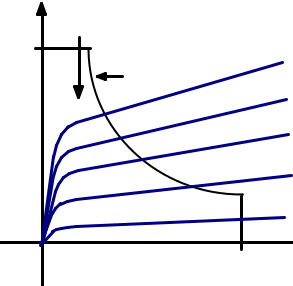
\includegraphics[width=1.36in,height=1.32in]{./media/image1.png}
\end{figure}


%%%%%%%%%%%%%%%%%%%% Figure/Image No: 1 Ends here %%%%%%%%%%%%%%%%%%%%

\par

\begin{adjustwidth}{2.58in}{0.0in}
{\fontsize{4pt}{4.8pt}\selectfont C\par}\par

\end{adjustwidth}

\begin{adjustwidth}{2.79in}{0.0in}
{\fontsize{4pt}{4.8pt}\selectfont \textit{SOA}\par}\par

\end{adjustwidth}

\begin{enumerate}
	\item {\fontsize{3pt}{3.6pt}\selectfont C Max\par}
\end{enumerate}\par


\vspace{\baselineskip}
\begin{adjustwidth}{1.79in}{0.0in}
\begin{Center}
\textit{\textsuperscript{P}}{\fontsize{3pt}{3.6pt}\selectfont CE Max\par}
\end{Center}\par

\end{adjustwidth}


\vspace{\baselineskip}

\vspace{\baselineskip}

\vspace{\baselineskip}
\begin{adjustwidth}{3.82in}{0.0in}
{\fontsize{4pt}{4.8pt}\selectfont \textit{I }\textsubscript{B}\textit{=0}\par}\par

\end{adjustwidth}



%%%%%%%%%%%%%%%%%%%% Figure/Image No: 2 starts here %%%%%%%%%%%%%%%%%%%%

\begin{figure}[H]
	\begin{Center}
		
\includegraphics[width=0.08in,height=0.06in]{./media/image2.png}
	\end{Center}
\end{figure}


%%%%%%%%%%%%%%%%%%%% Figure/Image No: 2 Ends here %%%%%%%%%%%%%%%%%%%%

\begin{adjustwidth}{3.82in}{0.0in}
\textit{\textsuperscript{ v}}\textsubscript{CE}\par

\end{adjustwidth}

\begin{adjustwidth}{3.49in}{0.0in}
\textit{\textsuperscript{V}}{\fontsize{4pt}{4.8pt}\selectfont CE Max\par}\par

\end{adjustwidth}


\vspace{\baselineskip}
\begin{adjustwidth}{0.0in}{0.01in}
\begin{Center}
Figure 1: Area Segura de Operación del Transistor.
\end{Center}\par

\end{adjustwidth}


\vspace{\baselineskip}
\begin{adjustwidth}{1.07in}{0.0in}
{\fontsize{9pt}{10.8pt}\selectfont La corriente i\textsubscript{C} y el voltaje V\textsubscript{CE} no podrán sobrepasar los máximos indicados.\par}\par

\end{adjustwidth}


\vspace{\baselineskip}

\vspace{\baselineskip}
\begin{adjustwidth}{0.0in}{0.01in}
\begin{Center}
{\fontsize{8pt}{9.6pt}\selectfont 1\par}
\end{Center}\par

\end{adjustwidth}


\vspace{\baselineskip}

\vspace{\baselineskip}

\vspace{\baselineskip}

\vspace{\baselineskip}
\begin{itemize}
	\item {\fontsize{14pt}{16.8pt}\selectfont \textcolor[HTML]{5C2D91}{Clasificación de los amplificadores de potencia}\par}
\end{itemize}\par


\vspace{\baselineskip}
\begin{adjustwidth}{0.86in}{0.88in}
\begin{justify}
Existen cuatro clasificaciones básicas de amplificadores de potencia: A, AB, B y C. En clase A, el amplificador está polarizado de tal forma que la corriente por el colector sustituye durante el ciclo completo de la señal de entrada. Para clase AB, la polarización del amplificador es de tal forma que la corriente de colector solamente sustituye para un lapso menor a los 360\textsuperscript{o} y mayor a los 180\textsuperscript{o} de la onda correspondiente. Para el funcionamiento en clase B, la corriente incluirá solo durante 180\textsuperscript{o} de la onda de entrada. Finalmente, para funcionamiento en clase C, el dispositivo conducirá durante un periodo inferior a los 180\textsuperscript{o} correspondiente a la onda de entrada. La Fig. 2, muestra el comportamiento del dispositivo en las distintas clases.
\end{justify}\par

\end{adjustwidth}


\vspace{\baselineskip}


%%%%%%%%%%%%%%%%%%%% Table No: 1 starts here %%%%%%%%%%%%%%%%%%%%


\begin{table}[H]
 			\centering
\begin{tabular}{p{0.27in}p{1.26in}p{0.81in}}
%row no:1
\multicolumn{1}{p{0.27in}}{\textit{\textsuperscript{v}}{\fontsize{6pt}{7.2pt}\selectfont \textit{BE}}} & 
\multicolumn{1}{p{1.26in}}{\textit{\textsuperscript{i}}{\fontsize{6pt}{7.2pt}\selectfont \textit{ C}}} & 
\multicolumn{1}{p{0.81in}}{} \\
\hhline{~~~}
%row no:2
\multicolumn{1}{p{0.27in}}{} & 
\multicolumn{1}{p{1.26in}}{{\fontsize{6pt}{7.2pt}\selectfont Clase A}} & 
\multicolumn{1}{p{0.81in}}{} \\
\hhline{~~~}
%row no:3
\multicolumn{1}{p{0.27in}}{} & 
\multicolumn{1}{p{1.26in}}{{\fontsize{6pt}{7.2pt}\selectfont }} & 
\multicolumn{1}{p{0.81in}}{{\fontsize{6pt}{7.2pt}\selectfont }} \\
\hhline{~~~}
%row no:4
\multicolumn{1}{p{0.27in}}{} & 
\multicolumn{1}{p{1.26in}}{{\fontsize{6pt}{7.2pt}\selectfont Clase B}} & 
\multicolumn{1}{p{0.81in}}{} \\
\hhline{~~~}
%row no:5
\multicolumn{1}{p{0.27in}}{} & 
\multicolumn{1}{p{1.26in}}{{\fontsize{6pt}{7.2pt}\selectfont }} & 
\multicolumn{1}{p{0.81in}}{} \\
\hhline{~~~}
%row no:6
\multicolumn{1}{p{0.27in}}{} & 
\multicolumn{1}{p{1.26in}}{{\fontsize{6pt}{7.2pt}\selectfont Clase AB}} & 
\multicolumn{1}{p{0.81in}}{{\fontsize{5pt}{6.0pt}\selectfont Conducción > {\fontsize{6pt}{7.2pt}\selectfont }}} \\
\hhline{~~~}
%row no:7
\multicolumn{1}{p{0.27in}}{} & 
\multicolumn{1}{p{1.26in}}{{\fontsize{6pt}{7.2pt}\selectfont }} & 
\multicolumn{1}{p{0.81in}}{{\fontsize{6pt}{7.2pt}\selectfont }} \\
\hhline{~~~}
%row no:8
\multicolumn{1}{p{0.27in}}{} & 
\multicolumn{1}{p{1.26in}}{\multirow{1}{*}{\begin{tabular}{p{1.26in}}{\fontsize{6pt}{7.2pt}\selectfont Clase C}\\\end{tabular}}} & 
\multicolumn{1}{p{0.81in}}{{\fontsize{5pt}{6.0pt}\selectfont Conducción < {\fontsize{6pt}{7.2pt}\selectfont }}} \\
\hhline{~~~}
%row no:9
\multicolumn{1}{p{0.27in}}{} & 
\multicolumn{1}{p{1.26in}}{} & 
\multicolumn{1}{p{0.81in}}{} \\
\hhline{~~~}
%row no:10
\multicolumn{1}{p{0.27in}}{} & 
\multicolumn{1}{p{1.26in}}{{\fontsize{6pt}{7.2pt}\selectfont }} & 
\multicolumn{1}{p{0.81in}}{} \\
\hhline{~~~}

\end{tabular}
 \end{table}


%%%%%%%%%%%%%%%%%%%% Table No: 1 ends here %%%%%%%%%%%%%%%%%%%%



%%%%%%%%%%%%%%%%%%%% Figure/Image No: 3 starts here %%%%%%%%%%%%%%%%%%%%

\begin{figure}[H]
\advance\leftskip 1.68in		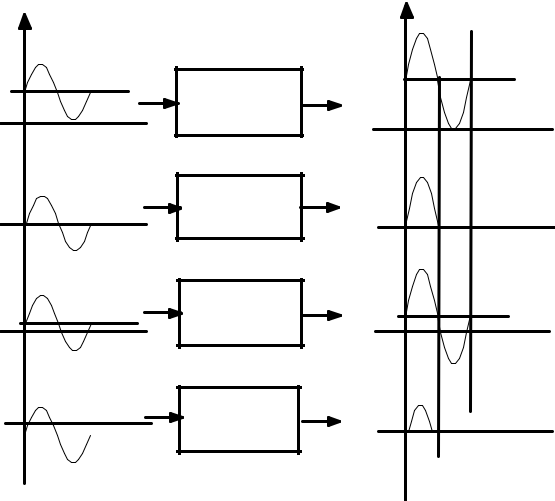
\includegraphics[width=2.57in,height=2.32in]{./media/image3.png}
\end{figure}


%%%%%%%%%%%%%%%%%%%% Figure/Image No: 3 Ends here %%%%%%%%%%%%%%%%%%%%

\par


\vspace{\baselineskip}

\vspace{\baselineskip}
\begin{adjustwidth}{0.0in}{0.01in}
\begin{Center}
Figure 2: Comportamiento para clase A, AB, B, C.
\end{Center}\par

\end{adjustwidth}


\vspace{\baselineskip}

\vspace{\baselineskip}
\begin{adjustwidth}{0.86in}{0.88in}
\begin{justify}
{\fontsize{9pt}{10.8pt}\selectfont Los amplificadores tipo AB y B usan configuraciones transistorizadas llamadas pushpull. Cada uno de estos amplificadores posee características de e$ \ldots $ ciencia y distorsión distintos, por lo cual, sus aplicación será a distintas áreas.\par}
\end{justify}\par

\end{adjustwidth}


\vspace{\baselineskip}
\begin{itemize}
	\item {\fontsize{14pt}{16.8pt}\selectfont \textcolor[HTML]{5C2D91}{Relaciones básicas en los amplificadores de potencia}\par}
\end{itemize}\par


\vspace{\baselineskip}
\begin{adjustwidth}{0.86in}{0.88in}
\begin{justify}
Para el análisis de los amplificadores de potencia se requiere de relaciones aso-ciadas a su funcionamiento y desempeño. Como el amplificador de potencia convierte la potencia de CC de la fuente de alimentación en una señal de potencia en la carga, la e$ \ldots $ ciencia de este proceso está dada por
\end{justify}\par

\end{adjustwidth}



%%%%%%%%%%%%%%%%%%%% Table No: 2 starts here %%%%%%%%%%%%%%%%%%%%


\begin{table}[H]
 			\centering
\begin{tabular}{p{1.42in}p{0.91in}}
%row no:1
\multicolumn{1}{p{1.42in}}{\textsuperscript{P}{\fontsize{7pt}{8.4pt}\selectfont L(CA)}} & 
\multicolumn{1}{p{0.91in}}{\multirow{1}{*}{\begin{tabular}{p{0.91in}}(1)\\\end{tabular}}} \\ 

\hhline{~~}
%row no:2
\multicolumn{1}{p{1.42in}}{\textsuperscript{=}\  P\textsubscript{CC}} & 
\multicolumn{1}{p{0.91in}}{} \\
\hhline{~~}

\end{tabular}
 \end{table}


%%%%%%%%%%%%%%%%%%%% Table No: 2 ends here %%%%%%%%%%%%%%%%%%%%

\par 
 \begin{tikzpicture}

\draw (3.16in,0.24in) -- (3.59in,0.24in); 

\end{tikzpicture}

\vspace{\baselineskip}
\begin{adjustwidth}{0.0in}{0.01in}
\begin{Center}
{\fontsize{8pt}{9.6pt}\selectfont 2\par}
\end{Center}\par

\end{adjustwidth}


\vspace{\baselineskip}

\vspace{\baselineskip}

\vspace{\baselineskip}

\vspace{\baselineskip}

\vspace{\baselineskip}
\begin{adjustwidth}{0.86in}{0.88in}
\begin{justify}
Donde es la eficiencia, P\textsubscript{L(CA)}, es la potencia media de señal en la carga y P\textsubscript{CC}, la potencia media de salida en la fuente de alimentación.
\end{justify}\par

\end{adjustwidth}


\vspace{\baselineskip}
\begin{adjustwidth}{0.86in}{0.88in}
\begin{justify}
La potencia media disipada en el dispositivo de amplificación, considerando un transistor bipolar como dispositivo de potencia, será
\end{justify}\par

\end{adjustwidth}


\vspace{\baselineskip}


%%%%%%%%%%%%%%%%%%%% Table No: 3 starts here %%%%%%%%%%%%%%%%%%%%


\begin{table}[H]
 			\centering
\begin{tabular}{p{1.7in}p{0.81in}}
%row no:1
\multicolumn{1}{p{1.7in}}{P\textsubscript{CE} = P\textsubscript{CC}\ \  P\textsubscript{L}} & 
\multicolumn{1}{p{0.81in}}{(2)} \\
\hhline{~~}

\end{tabular}
 \end{table}


%%%%%%%%%%%%%%%%%%%% Table No: 3 ends here %%%%%%%%%%%%%%%%%%%%

\begin{adjustwidth}{1.07in}{0.0in}
{\fontsize{9pt}{10.8pt}\selectfont Donde\  P\textsubscript{CE} es la disipación media de colector, P\textsubscript{L} es la potencia total, es\par}\par

\end{adjustwidth}

\begin{adjustwidth}{0.86in}{0.0in}
\textsuperscript{decir,}{\fontsize{6pt}{7.2pt}\selectfont  \textsuperscript{P}L \textsuperscript{=} \textsuperscript{P}L(DC)\textsuperscript{+} \textsuperscript{P}L(CA)\textsuperscript{.}\par}\par

\end{adjustwidth}

\begin{adjustwidth}{1.07in}{0.0in}
{\fontsize{9pt}{10.8pt}\selectfont Para la determinación de las potencias se usará (3), donde p es la potencia\par}\par

\end{adjustwidth}


\vspace{\baselineskip}


%%%%%%%%%%%%%%%%%%%% Table No: 4 starts here %%%%%%%%%%%%%%%%%%%%


\begin{table}[H]
 			\centering
\begin{tabular}{p{3.88in}p{0.48in}}
%row no:1
\multicolumn{1}{p{3.88in}}{instantánea, v e i son el voltaje y la corriente instantáneos.} & 
\multicolumn{1}{p{0.48in}}{} \\
\hhline{~~}
%row no:2
\multicolumn{1}{p{3.88in}}{p = vi} & 
\multicolumn{1}{p{0.48in}}{(3)} \\
\hhline{~~}

\end{tabular}
 \end{table}


%%%%%%%%%%%%%%%%%%%% Table No: 4 ends here %%%%%%%%%%%%%%%%%%%%


\vspace{\baselineskip}
\begin{adjustwidth}{0.86in}{0.88in}
\begin{justify}
{\fontsize{9pt}{10.8pt}\selectfont Sean v e i formas de onda periódica, con componente continua (la cual puede ser cero) y una componente de corriente alterna, no necesariamente sinusoidal\par}
\end{justify}\par

\end{adjustwidth}


\vspace{\baselineskip}


%%%%%%%%%%%%%%%%%%%% Table No: 5 starts here %%%%%%%%%%%%%%%%%%%%


\begin{table}[H]
 			\centering
\begin{tabular}{p{-0.06in}p{0.05in}p{1.36in}p{0.8in}}
%row no:1
\multicolumn{1}{p{-0.06in}}{v} & 
\multicolumn{1}{p{0.05in}}{=} & 
\multicolumn{1}{p{1.36in}}{\textsuperscript{V}{\fontsize{7pt}{8.4pt}\selectfont DC \textsuperscript{+} \textsuperscript{v}CA}} & 
\multicolumn{1}{p{0.8in}}{(4)} \\
\hhline{~~~~}
%row no:2
\multicolumn{1}{p{-0.06in}}{i} & 
\multicolumn{1}{p{0.05in}}{=} & 
\multicolumn{1}{p{1.36in}}{\textsuperscript{I}{\fontsize{7pt}{8.4pt}\selectfont DC \textsuperscript{+} \textsuperscript{i}CA}} & 
\multicolumn{1}{p{0.8in}}{(5)} \\
\hhline{~~~~}

\end{tabular}
 \end{table}


%%%%%%%%%%%%%%%%%%%% Table No: 5 ends here %%%%%%%%%%%%%%%%%%%%

\begin{adjustwidth}{1.07in}{0.0in}
Luego la potencia media en un periodo T será\par

\end{adjustwidth}


\vspace{\baselineskip}


%%%%%%%%%%%%%%%%%%%% Table No: 6 starts here %%%%%%%%%%%%%%%%%%%%


\begin{table}[H]
 			\centering
\begin{tabular}{p{0.22in}p{-0.12in}p{-0.05in}p{0.12in}p{0.02in}p{-0.05in}p{-0.17in}p{-0.12in}p{-0.14in}p{1.16in}p{0.48in}}
%row no:1
\multicolumn{1}{p{0.22in}}{} & 
\multicolumn{2}{p{0.04in}}{\multirow{1}{*}{\begin{tabular}{p{0.04in}}1\\\end{tabular}}} & 
\multicolumn{1}{p{0.12in}}{{\fontsize{7pt}{8.4pt}\selectfont 2}} & 
\multicolumn{1}{p{0.02in}}{} & 
\multicolumn{1}{p{-0.05in}}{} & 
\multicolumn{1}{p{-0.17in}}{} & 
\multicolumn{1}{p{-0.12in}}{} & 
\multicolumn{1}{p{-0.14in}}{} & 
\multicolumn{1}{p{1.16in}}{} & 
\multicolumn{1}{p{0.48in}}{} \\
\hhline{~~~~~~~~~~~}
%row no:2
\multicolumn{1}{p{0.22in}}{\multirow{1}{*}{\begin{tabular}{p{0.22in}}P\  =\\\end{tabular}}} & 
\multicolumn{2}{p{0.04in}}{} & 
\multicolumn{1}{p{0.12in}}{\multirow{1}{*}{\begin{tabular}{p{0.12in}}Z\textsubscript{0}\\\end{tabular}}} & 
\multicolumn{3}{p{0.2in}}{\multirow{1}{*}{\begin{tabular}{p{0.2in}}p d!t\\\end{tabular}}} & 
\multicolumn{1}{p{-0.12in}}{} & 
\multicolumn{1}{p{-0.14in}}{} & 
\multicolumn{1}{p{1.16in}}{} & 
\multicolumn{1}{p{0.48in}}{} \\
\hhline{~~~~~~~~~~~}
%row no:3
\multicolumn{1}{p{0.22in}}{} & 
\multicolumn{1}{p{-0.12in}}{} & 
\multicolumn{1}{p{-0.05in}}{} & 
\multicolumn{1}{p{0.12in}}{} & 
\multicolumn{3}{p{0.2in}}{} & 
\multicolumn{1}{p{-0.12in}}{} & 
\multicolumn{1}{p{-0.14in}}{} & 
\multicolumn{1}{p{1.16in}}{} & 
\multicolumn{1}{p{0.48in}}{} \\
\hhline{~~~~~~~~~~~}
%row no:4
\multicolumn{1}{p{0.22in}}{} & 
\multicolumn{2}{p{0.04in}}{2} & 
\multicolumn{1}{p{0.12in}}{} & 
\multicolumn{3}{p{0.2in}}{} & 
\multicolumn{1}{p{-0.12in}}{\multirow{1}{*}{\begin{tabular}{p{-0.12in}}{\fontsize{9pt}{10.8pt}\selectfont Z}\\\end{tabular}}} & 
\multicolumn{1}{p{-0.14in}}{} & 
\multicolumn{1}{p{1.16in}}{} & 
\multicolumn{1}{p{0.48in}}{} \\
\hhline{~~~~~~~~~~~}
%row no:5
\multicolumn{1}{p{0.22in}}{} & 
\multicolumn{1}{p{-0.12in}}{} & 
\multicolumn{1}{p{-0.05in}}{} & 
\multicolumn{1}{p{0.12in}}{} & 
\multicolumn{1}{p{0.02in}}{} & 
\multicolumn{1}{p{-0.05in}}{\multirow{1}{*}{\begin{tabular}{p{-0.05in}}1\\\end{tabular}}} & 
\multicolumn{1}{p{-0.17in}}{} & 
\multicolumn{1}{p{-0.12in}}{} & 
\multicolumn{1}{p{-0.14in}}{} & 
\multicolumn{1}{p{1.16in}}{{\fontsize{7pt}{8.4pt}\selectfont 2}} & 
\multicolumn{1}{p{0.48in}}{} \\
\hhline{~~~~~~~~~~~}
%row no:6
\multicolumn{1}{p{0.22in}}{\multirow{1}{*}{\begin{tabular}{p{0.22in}}=\\\end{tabular}}} & 
\multicolumn{4}{p{0.58in}}{\multirow{1}{*}{\begin{tabular}{p{0.58in}}\Centering \textsuperscript{V}{\fontsize{7pt}{8.4pt}\selectfont DC\textsuperscript{I}DC \textsuperscript{+}}\\\end{tabular}}} & 
\multicolumn{1}{p{-0.05in}}{} & 
\multicolumn{1}{p{-0.17in}}{} & 
\multicolumn{1}{p{-0.12in}}{} & 
\multicolumn{1}{p{-0.14in}}{} & 
\multicolumn{1}{p{1.16in}}{\multirow{1}{*}{\begin{tabular}{p{1.16in}}v\textsubscript{CA}i\textsubscript{CA}d!t\\\end{tabular}}} & 
\multicolumn{1}{p{0.48in}}{\multirow{1}{*}{\begin{tabular}{p{0.48in}}(6)\\\end{tabular}}} \\ 

\hhline{~~~~~~~~~~~}
%row no:7
\multicolumn{1}{p{0.22in}}{} & 
\multicolumn{4}{p{0.58in}}{} & 
\multicolumn{1}{p{-0.05in}}{} & 
\multicolumn{1}{p{-0.17in}}{} & 
\multicolumn{1}{p{-0.12in}}{} & 
\multicolumn{1}{p{-0.14in}}{} & 
\multicolumn{1}{p{1.16in}}{} & 
\multicolumn{1}{p{0.48in}}{} \\
\hhline{~~~~~~~~~~~}
%row no:8
\multicolumn{1}{p{0.22in}}{} & 
\multicolumn{4}{p{0.58in}}{} & 
\multicolumn{2}{p{-0.02in}}{2} & 
\multicolumn{1}{p{-0.12in}}{} & 
\multicolumn{1}{p{-0.14in}}{{\fontsize{7pt}{8.4pt}\selectfont 0}} & 
\multicolumn{1}{p{1.16in}}{} & 
\multicolumn{1}{p{0.48in}}{} \\
\hhline{~~~~~~~~~~~}
%row no:9
\multicolumn{1}{p{0.22in}}{} & 
\multicolumn{1}{p{-0.12in}}{} & 
\multicolumn{1}{p{-0.05in}}{} & 
\multicolumn{1}{p{0.12in}}{\Centering "} & 
\multicolumn{1}{p{0.02in}}{} & 
\multicolumn{1}{p{-0.05in}}{} & 
\multicolumn{1}{p{-0.17in}}{} & 
\multicolumn{1}{p{-0.12in}}{} & 
\multicolumn{1}{p{-0.14in}}{} & 
\multicolumn{1}{p{1.16in}}{"} & 
\multicolumn{1}{p{0.48in}}{} \\
\hhline{~~~~~~~~~~~}
%row no:10
\multicolumn{1}{p{0.22in}}{} & 
\multicolumn{1}{p{-0.12in}}{} & 
\multicolumn{1}{p{-0.05in}}{} & 
\multicolumn{1}{p{0.12in}}{\Centering \textsuperscript{P}{\fontsize{7pt}{8.4pt}\selectfont CC}} & 
\multicolumn{1}{p{0.02in}}{} & 
\multicolumn{1}{p{-0.05in}}{} & 
\multicolumn{1}{p{-0.17in}}{} & 
\multicolumn{1}{p{-0.12in}}{} & 
\multicolumn{1}{p{-0.14in}}{} & 
\multicolumn{1}{p{1.16in}}{\textsuperscript{P}{\fontsize{7pt}{8.4pt}\selectfont CA}} & 
\multicolumn{1}{p{0.48in}}{} \\
\hhline{~~~~~~~~~~~}

\end{tabular}
 \end{table}


%%%%%%%%%%%%%%%%%%%% Table No: 6 ends here %%%%%%%%%%%%%%%%%%%%

\begin{adjustwidth}{0.86in}{0.88in}
\begin{justify}
Donde, P\textsubscript{CC} es la contribución de la componente continua y P\textsubscript{CA} es la contribución de la componente alterna a la potencia media. Considerando v\textsubscript{CA} (t) = V\textsubscript{m} cos !t y i\textsubscript{CA} (t) = I\textsubscript{m} cos !t; reemplazando en (6), se tiene
\end{justify}\par

\end{adjustwidth}


\vspace{\baselineskip}


%%%%%%%%%%%%%%%%%%%% Table No: 7 starts here %%%%%%%%%%%%%%%%%%%%


\begin{table}[H]
 			\centering
\begin{tabular}{p{0.56in}p{-0.13in}p{-0.09in}p{-0.13in}p{0.4in}p{-0.05in}p{-0.01in}p{0.34in}p{-0.09in}p{-0.13in}p{-0.09in}p{-0.13in}p{-0.12in}p{0.16in}p{0.63in}p{0.22in}}
%row no:1
\multicolumn{1}{p{0.56in}}{} & 
\multicolumn{1}{p{-0.13in}}{} & 
\multicolumn{1}{p{-0.09in}}{} & 
\multicolumn{3}{p{0.62in}}{\multirow{1}{*}{\begin{tabular}{p{0.62in}}1\\\end{tabular}}} & 
\multicolumn{9}{p{2.18in}}{{\fontsize{7pt}{8.4pt}\selectfont 2}} & 
\multicolumn{1}{p{0.22in}}{} \\
\hhline{~~~~~~~~~~~~~~~~}
%row no:2
\multicolumn{1}{p{0.56in}}{} & 
\multicolumn{1}{p{-0.13in}}{} & 
\multicolumn{1}{p{-0.09in}}{} & 
\multicolumn{3}{p{0.62in}}{} & 
\multicolumn{1}{p{-0.01in}}{\multirow{1}{*}{\begin{tabular}{p{-0.01in}}Z\textsubscript{0}\\\end{tabular}}} & 
\multicolumn{1}{p{0.34in}}{} & 
\multicolumn{1}{p{-0.09in}}{} & 
\multicolumn{1}{p{-0.13in}}{} & 
\multicolumn{1}{p{-0.09in}}{} & 
\multicolumn{1}{p{-0.13in}}{} & 
\multicolumn{1}{p{-0.12in}}{} & 
\multicolumn{1}{p{0.16in}}{} & 
\multicolumn{1}{p{0.63in}}{} & 
\multicolumn{1}{p{0.22in}}{} \\
\hhline{~~~~~~~~~~~~~~~~}
%row no:3
\multicolumn{2}{p{0.63in}}{\multirow{1}{*}{\begin{tabular}{p{0.63in}}P\  =\\\end{tabular}}} & 
\multicolumn{3}{p{0.58in}}{\multirow{1}{*}{\begin{tabular}{p{0.58in}}\textsuperscript{V}{\fontsize{7pt}{8.4pt}\selectfont DC\textsuperscript{I}DC \textsuperscript{+}}\\\end{tabular}}} & 
\multicolumn{1}{p{-0.05in}}{} & 
\multicolumn{1}{p{-0.01in}}{} & 
\multicolumn{8}{p{1.98in}}{\multirow{1}{*}{\begin{tabular}{p{1.98in}}[(V\textsubscript{m} cos !t) (I\textsubscript{m} cos !t)] d!t =\\\end{tabular}}} & 
\multicolumn{1}{p{0.22in}}{} \\
\hhline{~~~~~~~~~~~~~~~~}
%row no:4
\multicolumn{2}{p{0.63in}}{} & 
\multicolumn{3}{p{0.58in}}{} & 
\multicolumn{1}{p{-0.05in}}{2} & 
\multicolumn{1}{p{-0.01in}}{} & 
\multicolumn{8}{p{1.98in}}{} & 
\multicolumn{1}{p{0.22in}}{} \\
\hhline{~~~~~~~~~~~~~~~~}
%row no:5
\multicolumn{2}{p{0.63in}}{\multirow{1}{*}{\begin{tabular}{p{0.63in}}=\\\end{tabular}}} & 
\multicolumn{3}{p{0.58in}}{\multirow{1}{*}{\begin{tabular}{p{0.58in}}\textsuperscript{V}{\fontsize{6pt}{7.2pt}\selectfont DC\textsuperscript{I}DC \textsuperscript{+}}\\\end{tabular}}} & 
\multicolumn{2}{p{0.15in}}{{\fontsize{9pt}{10.8pt}\selectfont V\textsubscript{m}I\textsubscript{m}}} & 
\multicolumn{6}{p{0.79in}}{\multirow{1}{*}{\begin{tabular}{p{0.79in}}= V\textsubscript{DC}I\textsubscript{DC} +\\\end{tabular}}} & 
\multicolumn{1}{p{0.16in}}{\Centering {\fontsize{9pt}{10.8pt}\selectfont V\textsubscript{m}I\textsubscript{m}}} & 
\multicolumn{1}{p{0.63in}}{\multirow{1}{*}{\begin{tabular}{p{0.63in}}\end{tabular}}} & 
\multicolumn{1}{p{0.22in}}{\multirow{1}{*}{\begin{tabular}{p{0.22in}}(7)\\\end{tabular}}} \\ 

\hhline{~~~~~~~~~~~~~~~~}
%row no:6
\multicolumn{2}{p{0.63in}}{} & 
\multicolumn{3}{p{0.58in}}{} & 
\multicolumn{2}{p{0.15in}}{\multirow{1}{*}{\begin{tabular}{p{0.15in}}2\\\end{tabular}}} & 
\multicolumn{6}{p{0.79in}}{} & 
\multicolumn{1}{p{0.16in}}{} & 
\multicolumn{1}{p{0.63in}}{} & 
\multicolumn{1}{p{0.22in}}{} \\
\hhline{~~~~~~~~~~~~~~~~}
%row no:7
\multicolumn{1}{p{0.56in}}{} & 
\multicolumn{1}{p{-0.13in}}{} & 
\multicolumn{1}{p{-0.09in}}{} & 
\multicolumn{1}{p{-0.13in}}{} & 
\multicolumn{1}{p{0.4in}}{} & 
\multicolumn{2}{p{0.15in}}{} & 
\multicolumn{7}{p{1.15in}}{2} & 
\multicolumn{1}{p{0.63in}}{} & 
\multicolumn{1}{p{0.22in}}{} \\
\hhline{~~~~~~~~~~~~~~~~}
%row no:8
\multicolumn{1}{p{0.56in}}{\multirow{1}{*}{\begin{tabular}{p{0.56in}}Como 2 = \textsuperscript{p}\\\end{tabular}}} & 
\multicolumn{1}{p{-0.13in}}{} & 
\multicolumn{1}{p{-0.09in}}{\multirow{1}{*}{\begin{tabular}{p{-0.09in}}p\\\end{tabular}}} & 
\multicolumn{1}{p{-0.13in}}{} & 
\multicolumn{2}{p{0.55in}}{\multirow{1}{*}{\begin{tabular}{p{0.55in}}; entonces\\\end{tabular}}} & 
\multicolumn{1}{p{-0.01in}}{} & 
\multicolumn{1}{p{0.34in}}{} & 
\multicolumn{1}{p{-0.09in}}{} & 
\multicolumn{1}{p{-0.13in}}{} & 
\multicolumn{1}{p{-0.09in}}{} & 
\multicolumn{1}{p{-0.13in}}{} & 
\multicolumn{1}{p{-0.12in}}{} & 
\multicolumn{1}{p{0.16in}}{} & 
\multicolumn{1}{p{0.63in}}{} & 
\multicolumn{1}{p{0.22in}}{} \\
\hhline{~~~~~~~~~~~~~~~~}
%row no:9
\multicolumn{1}{p{0.56in}}{} & 
\multicolumn{1}{p{-0.13in}}{2} & 
\multicolumn{1}{p{-0.09in}}{} & 
\multicolumn{1}{p{-0.13in}}{2} & 
\multicolumn{2}{p{0.55in}}{} & 
\multicolumn{1}{p{-0.01in}}{} & 
\multicolumn{1}{p{0.34in}}{} & 
\multicolumn{1}{p{-0.09in}}{} & 
\multicolumn{1}{p{-0.13in}}{} & 
\multicolumn{1}{p{-0.09in}}{} & 
\multicolumn{1}{p{-0.13in}}{} & 
\multicolumn{1}{p{-0.12in}}{} & 
\multicolumn{1}{p{0.16in}}{} & 
\multicolumn{1}{p{0.63in}}{} & 
\multicolumn{1}{p{0.22in}}{} \\
\hhline{~~~~~~~~~~~~~~~~}
%row no:10
\multicolumn{1}{p{0.56in}}{} & 
\multicolumn{1}{p{-0.13in}}{} & 
\multicolumn{1}{p{-0.09in}}{} & 
\multicolumn{1}{p{-0.13in}}{} & 
\multicolumn{1}{p{0.4in}}{} & 
\multicolumn{1}{p{-0.05in}}{} & 
\multicolumn{1}{p{-0.01in}}{} & 
\multicolumn{1}{p{0.34in}}{} & 
\multicolumn{7}{p{1.44in}}{\textsuperscript{V}{\fontsize{7pt}{8.4pt}\selectfont m\textsuperscript{I}m}} & 
\multicolumn{1}{p{0.22in}}{} \\
\hhline{~~~~~~~~~~~~~~~~}
%row no:11
\multicolumn{1}{p{0.56in}}{} & 
\multicolumn{1}{p{-0.13in}}{} & 
\multicolumn{1}{p{-0.09in}}{} & 
\multicolumn{1}{p{-0.13in}}{} & 
\multicolumn{4}{p{1.29in}}{\multirow{1}{*}{\begin{tabular}{p{1.29in}}P\ \ =  V\textsubscript{DC}I\textsubscript{DC} +\\\end{tabular}}} & 
\multicolumn{1}{p{-0.09in}}{\multirow{1}{*}{\begin{tabular}{p{-0.09in}}p\\\end{tabular}}} & 
\multicolumn{1}{p{-0.13in}}{} & 
\multicolumn{1}{p{-0.09in}}{\multirow{1}{*}{\begin{tabular}{p{-0.09in}}p\\\end{tabular}}} & 
\multicolumn{1}{p{-0.13in}}{} & 
\multicolumn{3}{p{1.08in}}{} & 
\multicolumn{1}{p{0.22in}}{} \\
\hhline{~~~~~~~~~~~~~~~~}
%row no:12
\multicolumn{1}{p{0.56in}}{} & 
\multicolumn{1}{p{-0.13in}}{} & 
\multicolumn{1}{p{-0.09in}}{} & 
\multicolumn{1}{p{-0.13in}}{} & 
\multicolumn{4}{p{1.29in}}{} & 
\multicolumn{1}{p{-0.09in}}{} & 
\multicolumn{1}{p{-0.13in}}{2} & 
\multicolumn{1}{p{-0.09in}}{} & 
\multicolumn{1}{p{-0.13in}}{2} & 
\multicolumn{1}{p{-0.12in}}{} & 
\multicolumn{1}{p{0.16in}}{} & 
\multicolumn{1}{p{0.63in}}{} & 
\multicolumn{1}{p{0.22in}}{} \\
\hhline{~~~~~~~~~~~~~~~~}
%row no:13
\multicolumn{1}{p{0.56in}}{} & 
\multicolumn{1}{p{-0.13in}}{} & 
\multicolumn{1}{p{-0.09in}}{} & 
\multicolumn{3}{p{0.62in}}{=} & 
\multicolumn{9}{p{2.18in}}{\textsuperscript{V}{\fontsize{7pt}{8.4pt}\selectfont DC\textsuperscript{I}DC \textsuperscript{+} \textsuperscript{V}rms\textsuperscript{I}rms}} & 
\multicolumn{1}{p{0.22in}}{(8)} \\
\hhline{~~~~~~~~~~~~~~~~}

\end{tabular}
 \end{table}


%%%%%%%%%%%%%%%%%%%% Table No: 7 ends here %%%%%%%%%%%%%%%%%%%%

\par 
 \begin{tikzpicture}

\draw (3.57in,0.5in) -- (3.94in,0.5in); 

\end{tikzpicture}

\vspace{\baselineskip}
\begin{adjustwidth}{0.0in}{0.01in}
\begin{Center}
{\fontsize{8pt}{9.6pt}\selectfont 3\par}
\end{Center}\par

\end{adjustwidth}


\vspace{\baselineskip}

\vspace{\baselineskip}

\vspace{\baselineskip}

\vspace{\baselineskip}

\vspace{\baselineskip}
\begin{adjustwidth}{0.86in}{0.88in}
\begin{justify}
Cuando una señal de corriente periódica tiene componente continua el valor rms de la forma de onda se expresa como
\end{justify}\par

\end{adjustwidth}


\vspace{\baselineskip}
\begin{adjustwidth}{2.42in}{0.0in}
q\par

\end{adjustwidth}

\par 
 \begin{tikzpicture}

\draw (2.55in,0.05in) -- (4.53in,0.05in); 
\end{tikzpicture}


%%%%%%%%%%%%%%%%%%%% Table No: 8 starts here %%%%%%%%%%%%%%%%%%%%


\begin{table}[H]
 			\centering
\begin{tabular}{p{0.65in}p{0.29in}p{0.27in}p{1.02in}p{0.44in}}
%row no:1
\multicolumn{1}{p{0.65in}}{{\fontsize{8pt}{9.6pt}\selectfont I\textsubscript{rms}\ =\   I\textsuperscript{2}}} & 
\multicolumn{1}{p{0.29in}}{{\fontsize{8pt}{9.6pt}\selectfont + I\textsuperscript{2}}} & 
\multicolumn{1}{p{0.27in}}{{\fontsize{8pt}{9.6pt}\selectfont + I\textsuperscript{2}}} & 
\multicolumn{1}{p{1.02in}}{{\fontsize{8pt}{9.6pt}\selectfont + ::: + I\textsuperscript{2}}} & 
\multicolumn{1}{p{0.44in}}{(9)} \\
\hhline{~~~~~}
%row no:2
\multicolumn{1}{p{0.65in}}{{\fontsize{7pt}{8.4pt}\selectfont DC}} & 
\multicolumn{1}{p{0.29in}}{\textsuperscript{1}{\fontsize{5pt}{6.0pt}\selectfont rms}} & 
\multicolumn{1}{p{0.27in}}{\textsuperscript{2}{\fontsize{5pt}{6.0pt}\selectfont rms}} & 
\multicolumn{1}{p{1.02in}}{\textsuperscript{n}{\fontsize{5pt}{6.0pt}\selectfont rms}} & 
\multicolumn{1}{p{0.44in}}{} \\
\hhline{~~~~~}

\end{tabular}
 \end{table}


%%%%%%%%%%%%%%%%%%%% Table No: 8 ends here %%%%%%%%%%%%%%%%%%%%

\begin{adjustwidth}{0.86in}{0.88in}
\begin{justify}
Donde I\textsubscript{DC}, es la componente continua de la señal, I\textsubscript{1rms} es el primer ar-mónico de la señal, I\textsubscript{nrms} es el enésimo armónico de la señal. Para el caso de una señal sinusoidal con componente continua será
\end{justify}\par

\end{adjustwidth}


\vspace{\baselineskip}
\begin{adjustwidth}{0.0in}{0.24in}
\begin{Center}
q
\end{Center}\par

\end{adjustwidth}

\par 
 \begin{tikzpicture}

\draw (3.2in,0.05in) -- (3.89in,0.05in); 

\end{tikzpicture}
\begin{adjustwidth}{0.0in}{0.88in}
\begin{FlushRight}
{\fontsize{9pt}{10.8pt}\selectfont I\textsubscript{rms} = \tabto{0.22in} \par}I\textsubscript{DC}\textsuperscript{2} + I\textsubscript{rms}\textsuperscript{2 \tabto{2.42in} }{\fontsize{9pt}{10.8pt}\selectfont (10)\par}
\end{FlushRight}\par

\end{adjustwidth}


\vspace{\baselineskip}
\begin{itemize}
	\item {\fontsize{14pt}{16.8pt}\selectfont \textcolor[HTML]{5C2D91}{El amplificador Clase A}\par}
\end{itemize}\par


\vspace{\baselineskip}
\begin{adjustwidth}{0.86in}{0.88in}
\begin{justify}
En operación clase A, el transistor reproduce toda la señal de entrada, la corriente de colector es distinta de cero todo el tiempo, lo cual se considera muy ineficiente, ya que para señal cero en la entrada, se tiene un I\textsubscript{CQ} > 0, luego el transistor disipa potencia.
\end{justify}\par

\end{adjustwidth}


\vspace{\baselineskip}
\begin{adjustwidth}{0.86in}{0.0in}
\textcolor[HTML]{5C2D91}{4.1 \tabto{1.26in} Amplificador Emisor común}\par

\end{adjustwidth}


\vspace{\baselineskip}
\begin{adjustwidth}{0.86in}{0.88in}
\begin{justify}
Sea la configuración de emisor común de la Fig. 3a, la cual funciona en clase A. Por simplicicidad se hace la resistencia de emisor R\textsubscript{E} = 0. Se selecciona R\textsubscript{L} para máxima potencia de salida, lo que implica que la recta de carga de CA debe pasar por la curva P\textsubscript{CEMAX} . El circuito equivalente de CC y CA se indica en la Fig. 3b-c.
\end{justify}\par

\end{adjustwidth}


\vspace{\baselineskip}


%%%%%%%%%%%%%%%%%%%% Table No: 9 starts here %%%%%%%%%%%%%%%%%%%%


\begin{table}[H]
 			\centering
\begin{tabular}{p{-0.02in}p{0.68in}p{1.18in}}
%row no:1
\multicolumn{1}{p{-0.02in}}{} & 
\multicolumn{1}{p{0.68in}}{{\fontsize{7pt}{8.4pt}\selectfont \textit{V}}} & 
\multicolumn{1}{p{1.18in}}{\textit{\textsuperscript{V}}{\fontsize{5pt}{6.0pt}\selectfont \textit{CC}}} \\
\hhline{~~~}
%row no:2
\multicolumn{1}{p{-0.02in}}{} & 
\multicolumn{1}{p{0.68in}}{{\fontsize{5pt}{6.0pt}\selectfont \textit{CC}}} & 
\multicolumn{1}{p{1.18in}}{} \\
\hhline{~~~}
%row no:3
\multicolumn{1}{p{-0.02in}}{\textit{\textsuperscript{R}}{\fontsize{5pt}{6.0pt}\selectfont \textit{L}}} & 
\multicolumn{1}{p{0.68in}}{{\fontsize{7pt}{8.4pt}\selectfont \textit{R\textsubscript{L}}}} & 
\multicolumn{1}{p{1.18in}}{{\fontsize{7pt}{8.4pt}\selectfont \textit{R\textsubscript{L}}}} \\
\hhline{~~~}

\end{tabular}
 \end{table}


%%%%%%%%%%%%%%%%%%%% Table No: 9 ends here %%%%%%%%%%%%%%%%%%%%



%%%%%%%%%%%%%%%%%%%% Figure/Image No: 4 starts here %%%%%%%%%%%%%%%%%%%%


\begin{figure}[H]	\begin{subfigure}		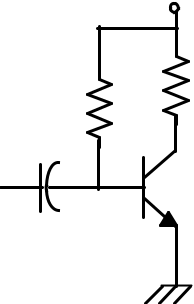
\includegraphics[width=0.28\textwidth]{./media/image4.png}
	\end{subfigure}
~	\begin{subfigure}		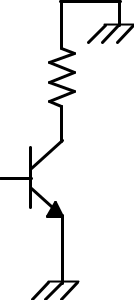
\includegraphics[width=0.28\textwidth]{./media/image5.png}
	\end{subfigure}
~	\begin{subfigure}		
\includegraphics[width=0.28\textwidth]{./media/image6.png}
	\end{subfigure}
~
\end{figure}


%%%%%%%%%%%%%%%%%%%% Figure/Image No: 4 Ends here %%%%%%%%%%%%%%%%%%%%

\par

\begin{adjustwidth}{1.61in}{0.0in}
\textit{\textsuperscript{R}}{\fontsize{5pt}{6.0pt}\selectfont \textit{B}\par}\par

\end{adjustwidth}


\vspace{\baselineskip}
\begin{adjustwidth}{1.26in}{0.0in}
{\fontsize{7pt}{8.4pt}\selectfont \textit{v\textsubscript{i}}\par}\par

\end{adjustwidth}


\vspace{\baselineskip}

\vspace{\baselineskip}

\vspace{\baselineskip}


%%%%%%%%%%%%%%%%%%%% Table No: 10 starts here %%%%%%%%%%%%%%%%%%%%


\begin{table}[H]
 			\centering
\begin{tabular}{p{0.22in}p{0.42in}p{-0.16in}p{-0.02in}p{-0.06in}p{-0.01in}p{0.61in}p{-0.14in}p{-0.16in}p{-0.06in}p{-0.1in}p{-0.16in}p{0.31in}}
%row no:1
\multicolumn{1}{p{0.22in}}{} & 
\multicolumn{1}{p{0.42in}}{\multirow{1}{*}{\begin{tabular}{p{0.42in}}{\fontsize{7pt}{8.4pt}\selectfont \textit{i \textsubscript{C}\ \  = \textsuperscript{\_}}}\\\end{tabular}}} & 
\multicolumn{2}{p{0.02in}}{\textit{\textsuperscript{v}}{\fontsize{5pt}{6.0pt}\selectfont \textit{ CE}}} & 
\multicolumn{2}{p{0.13in}}{{\fontsize{7pt}{8.4pt}\selectfont \textit{V}}} & 
\multicolumn{1}{p{0.61in}}{} & 
\multicolumn{2}{p{-0.1in}}{{\fontsize{7pt}{8.4pt}\selectfont \textit{v}}} & 
\multicolumn{1}{p{-0.06in}}{} & 
\multicolumn{1}{p{-0.1in}}{} & 
\multicolumn{2}{p{0.36in}}{{\fontsize{7pt}{8.4pt}\selectfont \textit{V}}} \\
\hhline{~~~~~~~~~~~~~}
%row no:2
\multicolumn{1}{p{0.22in}}{} & 
\multicolumn{1}{p{0.42in}}{} & 
\multicolumn{1}{p{-0.16in}}{} & 
\multicolumn{1}{p{-0.02in}}{} & 
\multicolumn{1}{p{-0.06in}}{{\fontsize{6pt}{7.2pt}\selectfont \textit{+}}} & 
\multicolumn{1}{p{-0.01in}}{{\fontsize{2pt}{2.4pt}\selectfont \textit{CC}}} & 
\multicolumn{1}{p{0.61in}}{{\fontsize{4pt}{4.8pt}\selectfont \textit{i \textsubscript{C}\ \  = \textsuperscript{\_}}}} & 
\multicolumn{1}{p{-0.14in}}{} & 
\multicolumn{1}{p{-0.16in}}{} & 
\multicolumn{1}{p{-0.06in}}{{\fontsize{2pt}{2.4pt}\selectfont \textit{CE}}} & 
\multicolumn{1}{p{-0.1in}}{{\fontsize{6pt}{7.2pt}\selectfont \textit{+}}} & 
\multicolumn{1}{p{-0.16in}}{} & 
\multicolumn{1}{p{0.31in}}{\textit{\textsuperscript{C E Q}}{\fontsize{4pt}{4.8pt}\selectfont \textit{ \textsubscript{+} I \textsubscript{CQ}}}} \\
\hhline{~~~~~~~~~~~~~}
%row no:3
\multicolumn{1}{p{0.22in}}{} & 
\multicolumn{1}{p{0.42in}}{} & 
\multicolumn{1}{p{-0.16in}}{} & 
\multicolumn{1}{p{-0.02in}}{{\fontsize{7pt}{8.4pt}\selectfont \textit{R\textsubscript{L}}}} & 
\multicolumn{1}{p{-0.06in}}{} & 
\multicolumn{1}{p{-0.01in}}{\textit{\textsuperscript{R}}{\fontsize{5pt}{6.0pt}\selectfont \textit{L}}} & 
\multicolumn{1}{p{0.61in}}{} & 
\multicolumn{1}{p{-0.14in}}{} & 
\multicolumn{3}{p{0.08in}}{{\fontsize{7pt}{8.4pt}\selectfont \textit{R\textsubscript{L}}}} & 
\multicolumn{1}{p{-0.16in}}{} & 
\multicolumn{1}{p{0.31in}}{{\fontsize{7pt}{8.4pt}\selectfont \textit{R\textsubscript{L}}}} \\
\hhline{~~~~~~~~~~~~~}
%row no:4
\multicolumn{1}{p{0.22in}}{{\fontsize{7pt}{8.4pt}\selectfont (a)}} & 
\multicolumn{1}{p{0.42in}}{} & 
\multicolumn{2}{p{0.02in}}{{\fontsize{7pt}{8.4pt}\selectfont (b)}} & 
\multicolumn{1}{p{-0.06in}}{} & 
\multicolumn{1}{p{-0.01in}}{} & 
\multicolumn{1}{p{0.61in}}{} & 
\multicolumn{1}{p{-0.14in}}{} & 
\multicolumn{1}{p{-0.16in}}{} & 
\multicolumn{2}{p{0.04in}}{{\fontsize{7pt}{8.4pt}\selectfont (c)}} & 
\multicolumn{1}{p{-0.16in}}{} & 
\multicolumn{1}{p{0.31in}}{} \\
\hhline{~~~~~~~~~~~~~}

\end{tabular}
 \end{table}


%%%%%%%%%%%%%%%%%%%% Table No: 10 ends here %%%%%%%%%%%%%%%%%%%%

\par 
 \begin{tikzpicture}

\draw (4.67in,0.38in) -- (4.85in,0.38in); 

\end{tikzpicture}

\vspace{\baselineskip}
\begin{adjustwidth}{0.0in}{0.01in}
\begin{Center}
Figure 3: (a) Emisor Común. (b) CC. (c) CA.
\end{Center}\par

\end{adjustwidth}


\vspace{\baselineskip}

\vspace{\baselineskip}
\begin{adjustwidth}{0.86in}{0.88in}
\begin{justify}
{\fontsize{9pt}{10.8pt}\selectfont Dependiendo del diseño, las rectas de carga estarán en dos puntos de operación Q; los cuales se intersectan con la curva P\textsubscript{CEMax;} de acuerdo a la Fig. 4a, se observa que I\textsubscript{C2} será la máxima corriente permitida para i\textsubscript{C} y V\textsubscript{CE1} será el\par}
\end{justify}\par

\end{adjustwidth}


\vspace{\baselineskip}

\vspace{\baselineskip}
\begin{adjustwidth}{0.0in}{0.01in}
\begin{Center}
{\fontsize{8pt}{9.6pt}\selectfont 4\par}
\end{Center}\par

\end{adjustwidth}


\vspace{\baselineskip}

\vspace{\baselineskip}

\vspace{\baselineskip}

\vspace{\baselineskip}

\vspace{\baselineskip}
\begin{adjustwidth}{0.86in}{0.88in}
\begin{justify}
máximo voltaje permitido para v\textsubscript{CE}: El óptimo elegido será el punto de reposo Q\textsubscript{1}, debido a que I\textsubscript{C1} < I\textsubscript{C2}, lo cual implica una menor corriente de colector, menor distorsión y una menor corriente de base requerida para obtener I\textsubscript{C}. Para que la realización sea factible, V\textsubscript{CE1} debe ser menor que V\textsubscript{CEO}, así se tomará que V\textsubscript{CE1} = V\textsubscript{CC}. Lo cual puede no ser necesariamente efectivo para otras configuraciones en clase A.
\end{justify}\par

\end{adjustwidth}


\vspace{\baselineskip}


%%%%%%%%%%%%%%%%%%%% Table No: 11 starts here %%%%%%%%%%%%%%%%%%%%


{
\scriptsize
\setlength\extrarowheight{3pt}
\begin{longtable}{p{-0.18in}p{-0.08in}p{-0.18in}p{-0.01in}p{-0.16in}p{-0.09in}p{-0.01in}p{-0.01in}p{-0.13in}p{-0.02in}p{-0.17in}p{0.01in}p{-0.18in}p{-0.16in}p{-0.06in}p{-0.09in}p{-0.08in}p{-0.18in}p{-0.09in}p{-0.06in}p{-0.1in}p{0.04in}p{-0.16in}p{0.02in}p{0.05in}p{-0.1in}}

\endfirsthead
\multicolumn{26}{c}{\textit{continued from previous page}}\hline
\endhead\hline
\multicolumn{26}{r}{\textit{continued on next page}} \\
\endfoot
\hline 
\endlastfoot%row no:1
\multicolumn{1}{p{-0.18in}}{\multirow{1}{*}{\begin{tabular}{p{-0.18in}}\end{tabular}}} & 
\multicolumn{1}{p{-0.08in}}{\multirow{1}{*}{\begin{tabular}{p{-0.08in}}\Centering {\fontsize{4pt}{4.8pt}\selectfont \textit{i}\textsubscript{C}}\\\end{tabular}}} & 
\multicolumn{1}{p{-0.18in}}{} & 
\multicolumn{1}{p{-0.01in}}{\multirow{1}{*}{\begin{tabular}{p{-0.01in}}\end{tabular}}} & 
\multicolumn{1}{p{-0.16in}}{\multirow{1}{*}{\begin{tabular}{p{-0.16in}}\end{tabular}}} & 
\multicolumn{1}{p{-0.09in}}{\multirow{1}{*}{\begin{tabular}{p{-0.09in}}\end{tabular}}} & 
\multicolumn{1}{p{-0.01in}}{\multirow{1}{*}{\begin{tabular}{p{-0.01in}}\end{tabular}}} & 
\multicolumn{1}{p{-0.01in}}{\multirow{1}{*}{\begin{tabular}{p{-0.01in}}\end{tabular}}} & 
\multicolumn{1}{p{-0.13in}}{\multirow{1}{*}{\begin{tabular}{p{-0.13in}}\end{tabular}}} & 
\multicolumn{1}{p{-0.02in}}{} & 
\multicolumn{1}{p{-0.17in}}{} & 
\multicolumn{1}{p{0.01in}}{} & 
\multicolumn{1}{p{-0.18in}}{} & 
\multicolumn{1}{p{-0.16in}}{} & 
\multicolumn{1}{p{-0.06in}}{} & 
\multicolumn{1}{p{-0.09in}}{} & 
\multicolumn{1}{p{-0.08in}}{\multirow{1}{*}{\begin{tabular}{p{-0.08in}}\Centering {\fontsize{4pt}{4.8pt}\selectfont \textit{i}\textsubscript{C}}\\\end{tabular}}} & 
\multicolumn{1}{p{-0.18in}}{} & 
\multicolumn{1}{p{-0.09in}}{} & 
\multicolumn{1}{p{-0.06in}}{} & 
\multicolumn{1}{p{-0.1in}}{} & 
\multicolumn{1}{p{0.04in}}{} & 
\multicolumn{1}{p{-0.16in}}{} & 
\multicolumn{1}{p{0.02in}}{} & 
\multicolumn{1}{p{0.05in}}{} & 
\multicolumn{1}{p{-0.1in}}{} \\
\hhline{~~~~~~~~~~~~~~~~~~~~~~~~~~}
%row no:2
\multicolumn{1}{p{-0.18in}}{} & 
\multicolumn{1}{p{-0.08in}}{} & 
\multicolumn{1}{p{-0.18in}}{\multirow{1}{*}{\begin{tabular}{p{-0.18in}}\end{tabular}}} & 
\multicolumn{1}{p{-0.01in}}{} & 
\multicolumn{1}{p{-0.16in}}{} & 
\multicolumn{1}{p{-0.09in}}{} & 
\multicolumn{1}{p{-0.01in}}{} & 
\multicolumn{1}{p{-0.01in}}{} & 
\multicolumn{1}{p{-0.13in}}{} & 
\multicolumn{1}{p{-0.02in}}{} & 
\multicolumn{1}{p{-0.17in}}{} & 
\multicolumn{1}{p{0.01in}}{} & 
\multicolumn{1}{p{-0.18in}}{} & 
\multicolumn{1}{p{-0.16in}}{} & 
\multicolumn{1}{p{-0.06in}}{} & 
\multicolumn{1}{p{-0.09in}}{\multirow{1}{*}{\begin{tabular}{p{-0.09in}}\end{tabular}}} & 
\multicolumn{1}{p{-0.08in}}{} & 
\multicolumn{1}{p{-0.18in}}{} & 
\multicolumn{1}{p{-0.09in}}{\multirow{1}{*}{\begin{tabular}{p{-0.09in}}\end{tabular}}} & 
\multicolumn{1}{p{-0.06in}}{\multirow{1}{*}{\begin{tabular}{p{-0.06in}}\end{tabular}}} & 
\multicolumn{1}{p{-0.1in}}{\multirow{1}{*}{\begin{tabular}{p{-0.1in}}\end{tabular}}} & 
\multicolumn{1}{p{0.04in}}{} & 
\multicolumn{1}{p{-0.16in}}{} & 
\multicolumn{1}{p{0.02in}}{} & 
\multicolumn{1}{p{0.05in}}{} & 
\multicolumn{1}{p{-0.1in}}{} \\
\hhline{~~~~~~~~~~~~~~~~~~~~~~~~~~}
%row no:3
\multicolumn{1}{p{-0.18in}}{} & 
\multicolumn{1}{p{-0.08in}}{} & 
\multicolumn{1}{p{-0.18in}}{} & 
\multicolumn{1}{p{-0.01in}}{} & 
\multicolumn{1}{p{-0.16in}}{} & 
\multicolumn{1}{p{-0.09in}}{} & 
\multicolumn{1}{p{-0.01in}}{} & 
\multicolumn{1}{p{-0.01in}}{} & 
\multicolumn{1}{p{-0.13in}}{} & 
\multicolumn{1}{p{-0.02in}}{} & 
\multicolumn{1}{p{-0.17in}}{} & 
\multicolumn{1}{p{0.01in}}{} & 
\multicolumn{1}{p{-0.18in}}{} & 
\multicolumn{1}{p{-0.16in}}{} & 
\multicolumn{1}{p{-0.06in}}{} & 
\multicolumn{1}{p{-0.09in}}{} & 
\multicolumn{1}{p{-0.08in}}{} & 
\multicolumn{1}{p{-0.18in}}{} & 
\multicolumn{1}{p{-0.09in}}{} & 
\multicolumn{1}{p{-0.06in}}{} & 
\multicolumn{1}{p{-0.1in}}{} & 
\multicolumn{1}{p{0.04in}}{} & 
\multicolumn{1}{p{-0.16in}}{} & 
\multicolumn{1}{p{0.02in}}{} & 
\multicolumn{1}{p{0.05in}}{} & 
\multicolumn{1}{p{-0.1in}}{} \\
\hhline{~~~~~~~~~~~~~~~~~~~~~~~~~~}
%row no:4
\multicolumn{1}{p{-0.18in}}{} & 
\multicolumn{1}{p{-0.08in}}{\multirow{1}{*}{\begin{tabular}{p{-0.08in}}\Centering \textit{\textsuperscript{I}}{\fontsize{3pt}{3.6pt}\selectfont C \textsubscript{2}}\\\end{tabular}}} & 
\multicolumn{1}{p{-0.18in}}{} & 
\multicolumn{1}{p{-0.01in}}{} & 
\multicolumn{1}{p{-0.16in}}{} & 
\multicolumn{1}{p{-0.09in}}{} & 
\multicolumn{3}{p{-0.01in}}{\multirow{1}{*}{\begin{tabular}{p{-0.01in}}\textit{\textsuperscript{P}}{\fontsize{3pt}{3.6pt}\selectfont CE Ma x}\\\end{tabular}}} & 
\multicolumn{1}{p{-0.02in}}{} & 
\multicolumn{1}{p{-0.17in}}{} & 
\multicolumn{1}{p{0.01in}}{} & 
\multicolumn{1}{p{-0.18in}}{} & 
\multicolumn{1}{p{-0.16in}}{} & 
\multicolumn{1}{p{-0.06in}}{} & 
\multicolumn{2}{p{-0.09in}}{\multirow{1}{*}{\begin{tabular}{p{-0.09in}}\textit{\textsuperscript{I}}{\fontsize{3pt}{3.6pt}\selectfont  C M a x}\\\end{tabular}}} & 
\multicolumn{1}{p{-0.18in}}{} & 
\multicolumn{1}{p{-0.09in}}{} & 
\multicolumn{1}{p{-0.06in}}{} & 
\multicolumn{1}{p{-0.1in}}{} & 
\multicolumn{1}{p{0.04in}}{\multirow{1}{*}{\begin{tabular}{p{0.04in}}\textit{\textsuperscript{P}}{\fontsize{3pt}{3.6pt}\selectfont CE Ma x}\\\end{tabular}}} & 
\multicolumn{1}{p{-0.16in}}{} & 
\multicolumn{1}{p{0.02in}}{} & 
\multicolumn{1}{p{0.05in}}{} & 
\multicolumn{1}{p{-0.1in}}{} \\
\hhline{~~~~~~~~~~~~~~~~~~~~~~~~~~}
%row no:5
\multicolumn{1}{p{-0.18in}}{} & 
\multicolumn{1}{p{-0.08in}}{} & 
\multicolumn{1}{p{-0.18in}}{} & 
\multicolumn{1}{p{-0.01in}}{} & 
\multicolumn{1}{p{-0.16in}}{} & 
\multicolumn{1}{p{-0.09in}}{} & 
\multicolumn{3}{p{-0.01in}}{} & 
\multicolumn{1}{p{-0.02in}}{} & 
\multicolumn{1}{p{-0.17in}}{} & 
\multicolumn{1}{p{0.01in}}{} & 
\multicolumn{1}{p{-0.18in}}{} & 
\multicolumn{1}{p{-0.16in}}{} & 
\multicolumn{1}{p{-0.06in}}{} & 
\multicolumn{2}{p{-0.09in}}{} & 
\multicolumn{1}{p{-0.18in}}{} & 
\multicolumn{1}{p{-0.09in}}{} & 
\multicolumn{1}{p{-0.06in}}{} & 
\multicolumn{1}{p{-0.1in}}{} & 
\multicolumn{1}{p{0.04in}}{} & 
\multicolumn{1}{p{-0.16in}}{} & 
\multicolumn{1}{p{0.02in}}{} & 
\multicolumn{1}{p{0.05in}}{} & 
\multicolumn{1}{p{-0.1in}}{} \\
\hhline{~~~~~~~~~~~~~~~~~~~~~~~~~~}
%row no:6
\multicolumn{1}{p{-0.18in}}{} & 
\multicolumn{1}{p{-0.08in}}{} & 
\multicolumn{1}{p{-0.18in}}{} & 
\multicolumn{1}{p{-0.01in}}{} & 
\multicolumn{1}{p{-0.16in}}{} & 
\multicolumn{1}{p{-0.09in}}{} & 
\multicolumn{3}{p{-0.01in}}{} & 
\multicolumn{1}{p{-0.02in}}{} & 
\multicolumn{1}{p{-0.17in}}{} & 
\multicolumn{1}{p{0.01in}}{} & 
\multicolumn{1}{p{-0.18in}}{} & 
\multicolumn{1}{p{-0.16in}}{} & 
\multicolumn{1}{p{-0.06in}}{} & 
\multicolumn{2}{p{-0.09in}}{} & 
\multicolumn{1}{p{-0.18in}}{} & 
\multicolumn{1}{p{-0.09in}}{} & 
\multicolumn{1}{p{-0.06in}}{} & 
\multicolumn{1}{p{-0.1in}}{} & 
\multicolumn{1}{p{0.04in}}{} & 
\multicolumn{1}{p{-0.16in}}{} & 
\multicolumn{1}{p{0.02in}}{} & 
\multicolumn{1}{p{0.05in}}{} & 
\multicolumn{1}{p{-0.1in}}{} \\
\hhline{~~~~~~~~~~~~~~~~~~~~~~~~~~}
%row no:7
\multicolumn{2}{p{0.18in}}{\multirow{1}{*}{\begin{tabular}{p{0.18in}}\textit{\textsuperscript{I}}{\fontsize{3pt}{3.6pt}\selectfont C \textsubscript{1}}\\\end{tabular}}} & 
\multicolumn{1}{p{-0.18in}}{} & 
\multicolumn{1}{p{-0.01in}}{} & 
\multicolumn{1}{p{-0.16in}}{} & 
\multicolumn{1}{p{-0.09in}}{} & 
\multicolumn{3}{p{-0.01in}}{} & 
\multicolumn{1}{p{-0.02in}}{} & 
\multicolumn{1}{p{-0.17in}}{} & 
\multicolumn{1}{p{0.01in}}{} & 
\multicolumn{1}{p{-0.18in}}{} & 
\multicolumn{1}{p{-0.16in}}{} & 
\multicolumn{1}{p{-0.06in}}{} & 
\multicolumn{1}{p{-0.09in}}{} & 
\multicolumn{1}{p{-0.08in}}{} & 
\multicolumn{1}{p{-0.18in}}{} & 
\multicolumn{1}{p{-0.09in}}{} & 
\multicolumn{1}{p{-0.06in}}{} & 
\multicolumn{1}{p{-0.1in}}{} & 
\multicolumn{1}{p{0.04in}}{} & 
\multicolumn{1}{p{-0.16in}}{} & 
\multicolumn{1}{p{0.02in}}{} & 
\multicolumn{1}{p{0.05in}}{} & 
\multicolumn{1}{p{-0.1in}}{} \\
\hhline{~~~~~~~~~~~~~~~~~~~~~~~~~~}
%row no:8
\multicolumn{2}{p{0.18in}}{} & 
\multicolumn{1}{p{-0.18in}}{} & 
\multicolumn{1}{p{-0.01in}}{} & 
\multicolumn{1}{p{-0.16in}}{} & 
\multicolumn{1}{p{-0.09in}}{} & 
\multicolumn{1}{p{-0.01in}}{} & 
\multicolumn{1}{p{-0.01in}}{} & 
\multicolumn{1}{p{-0.13in}}{} & 
\multicolumn{1}{p{-0.02in}}{} & 
\multicolumn{1}{p{-0.17in}}{} & 
\multicolumn{1}{p{0.01in}}{} & 
\multicolumn{1}{p{-0.18in}}{} & 
\multicolumn{1}{p{-0.16in}}{} & 
\multicolumn{1}{p{-0.06in}}{} & 
\multicolumn{1}{p{-0.09in}}{} & 
\multicolumn{1}{p{-0.08in}}{} & 
\multicolumn{1}{p{-0.18in}}{} & 
\multicolumn{1}{p{-0.09in}}{} & 
\multicolumn{1}{p{-0.06in}}{} & 
\multicolumn{1}{p{-0.1in}}{} & 
\multicolumn{1}{p{0.04in}}{} & 
\multicolumn{1}{p{-0.16in}}{} & 
\multicolumn{1}{p{0.02in}}{} & 
\multicolumn{1}{p{0.05in}}{} & 
\multicolumn{1}{p{-0.1in}}{} \\
\hhline{~~~~~~~~~~~~~~~~~~~~~~~~~~}
%row no:9
\multicolumn{1}{p{-0.18in}}{} & 
\multicolumn{1}{p{-0.08in}}{} & 
\multicolumn{1}{p{-0.18in}}{} & 
\multicolumn{1}{p{-0.01in}}{} & 
\multicolumn{1}{p{-0.16in}}{} & 
\multicolumn{1}{p{-0.09in}}{} & 
\multicolumn{3}{p{-0.01in}}{\Centering \textit{\textsuperscript{Q}}{\fontsize{3pt}{3.6pt}\selectfont 2}} & 
\multicolumn{1}{p{-0.02in}}{} & 
\multicolumn{1}{p{-0.17in}}{} & 
\multicolumn{1}{p{0.01in}}{} & 
\multicolumn{1}{p{-0.18in}}{} & 
\multicolumn{1}{p{-0.16in}}{} & 
\multicolumn{1}{p{-0.06in}}{} & 
\multicolumn{2}{p{-0.09in}}{\multirow{1}{*}{\begin{tabular}{p{-0.09in}}\Centering \textit{\textsuperscript{I}}{\fontsize{3pt}{3.6pt}\selectfont C Q}\\\end{tabular}}} & 
\multicolumn{1}{p{-0.18in}}{} & 
\multicolumn{1}{p{-0.09in}}{} & 
\multicolumn{1}{p{-0.06in}}{} & 
\multicolumn{1}{p{-0.1in}}{} & 
\multicolumn{1}{p{0.04in}}{{\fontsize{4pt}{4.8pt}\selectfont \textit{Q}}} & 
\multicolumn{1}{p{-0.16in}}{} & 
\multicolumn{1}{p{0.02in}}{} & 
\multicolumn{1}{p{0.05in}}{} & 
\multicolumn{1}{p{-0.1in}}{} \\
\hhline{~~~~~~~~~~~~~~~~~~~~~~~~~~}
%row no:10
\multicolumn{1}{p{-0.18in}}{} & 
\multicolumn{1}{p{-0.08in}}{} & 
\multicolumn{1}{p{-0.18in}}{} & 
\multicolumn{1}{p{-0.01in}}{} & 
\multicolumn{1}{p{-0.16in}}{} & 
\multicolumn{1}{p{-0.09in}}{} & 
\multicolumn{3}{p{-0.01in}}{\multirow{1}{*}{\begin{tabular}{p{-0.01in}}{\fontsize{4pt}{4.8pt}\selectfont \textit{Q}\textsubscript{1}}\\\end{tabular}}} & 
\multicolumn{1}{p{-0.02in}}{} & 
\multicolumn{1}{p{-0.17in}}{} & 
\multicolumn{1}{p{0.01in}}{} & 
\multicolumn{1}{p{-0.18in}}{} & 
\multicolumn{1}{p{-0.16in}}{} & 
\multicolumn{1}{p{-0.06in}}{} & 
\multicolumn{2}{p{-0.09in}}{} & 
\multicolumn{1}{p{-0.18in}}{} & 
\multicolumn{1}{p{-0.09in}}{} & 
\multicolumn{1}{p{-0.06in}}{} & 
\multicolumn{1}{p{-0.1in}}{} & 
\multicolumn{1}{p{0.04in}}{} & 
\multicolumn{1}{p{-0.16in}}{} & 
\multicolumn{1}{p{0.02in}}{} & 
\multicolumn{1}{p{0.05in}}{} & 
\multicolumn{1}{p{-0.1in}}{} \\
\hhline{~~~~~~~~~~~~~~~~~~~~~~~~~~}
%row no:11
\multicolumn{1}{p{-0.18in}}{} & 
\multicolumn{1}{p{-0.08in}}{} & 
\multicolumn{1}{p{-0.18in}}{} & 
\multicolumn{1}{p{-0.01in}}{} & 
\multicolumn{1}{p{-0.16in}}{} & 
\multicolumn{1}{p{-0.09in}}{} & 
\multicolumn{3}{p{-0.01in}}{} & 
\multicolumn{1}{p{-0.02in}}{} & 
\multicolumn{1}{p{-0.17in}}{} & 
\multicolumn{1}{p{0.01in}}{} & 
\multicolumn{1}{p{-0.18in}}{} & 
\multicolumn{1}{p{-0.16in}}{} & 
\multicolumn{1}{p{-0.06in}}{} & 
\multicolumn{1}{p{-0.09in}}{} & 
\multicolumn{1}{p{-0.08in}}{} & 
\multicolumn{1}{p{-0.18in}}{} & 
\multicolumn{1}{p{-0.09in}}{} & 
\multicolumn{1}{p{-0.06in}}{} & 
\multicolumn{1}{p{-0.1in}}{} & 
\multicolumn{1}{p{0.04in}}{} & 
\multicolumn{1}{p{-0.16in}}{} & 
\multicolumn{1}{p{0.02in}}{} & 
\multicolumn{1}{p{0.05in}}{} & 
\multicolumn{1}{p{-0.1in}}{} \\
\hhline{~~~~~~~~~~~~~~~~~~~~~~~~~~}
%row no:12
\multicolumn{1}{p{-0.18in}}{} & 
\multicolumn{1}{p{-0.08in}}{} & 
\multicolumn{1}{p{-0.18in}}{} & 
\multicolumn{1}{p{-0.01in}}{} & 
\multicolumn{1}{p{-0.16in}}{} & 
\multicolumn{1}{p{-0.09in}}{} & 
\multicolumn{1}{p{-0.01in}}{} & 
\multicolumn{1}{p{-0.01in}}{} & 
\multicolumn{1}{p{-0.13in}}{} & 
\multicolumn{1}{p{-0.02in}}{} & 
\multicolumn{1}{p{-0.17in}}{} & 
\multicolumn{1}{p{0.01in}}{} & 
\multicolumn{1}{p{-0.18in}}{} & 
\multicolumn{1}{p{-0.16in}}{} & 
\multicolumn{1}{p{-0.06in}}{} & 
\multicolumn{1}{p{-0.09in}}{} & 
\multicolumn{1}{p{-0.08in}}{} & 
\multicolumn{1}{p{-0.18in}}{} & 
\multicolumn{1}{p{-0.09in}}{} & 
\multicolumn{1}{p{-0.06in}}{} & 
\multicolumn{2}{p{-0.1in}}{} & 
\multicolumn{1}{p{-0.16in}}{} & 
\multicolumn{1}{p{0.02in}}{} & 
\multicolumn{1}{p{0.05in}}{} & 
\multicolumn{1}{p{-0.1in}}{} \\
\hhline{~~~~~~~~~~~~~~~~~~~~~~~~~~}
%row no:13
\multicolumn{1}{p{-0.18in}}{} & 
\multicolumn{1}{p{-0.08in}}{} & 
\multicolumn{1}{p{-0.18in}}{} & 
\multicolumn{1}{p{-0.01in}}{} & 
\multicolumn{1}{p{-0.16in}}{} & 
\multicolumn{1}{p{-0.09in}}{} & 
\multicolumn{1}{p{-0.01in}}{} & 
\multicolumn{1}{p{-0.01in}}{} & 
\multicolumn{1}{p{-0.13in}}{} & 
\multicolumn{1}{p{-0.02in}}{} & 
\multicolumn{1}{p{-0.17in}}{} & 
\multicolumn{1}{p{0.01in}}{} & 
\multicolumn{1}{p{-0.18in}}{} & 
\multicolumn{1}{p{-0.16in}}{} & 
\multicolumn{1}{p{-0.06in}}{} & 
\multicolumn{1}{p{-0.09in}}{} & 
\multicolumn{1}{p{-0.08in}}{} & 
\multicolumn{1}{p{-0.18in}}{} & 
\multicolumn{1}{p{-0.09in}}{} & 
\multicolumn{1}{p{-0.06in}}{} & 
\multicolumn{1}{p{-0.1in}}{} & 
\multicolumn{1}{p{0.04in}}{} & 
\multicolumn{1}{p{-0.16in}}{} & 
\multicolumn{1}{p{0.02in}}{} & 
\multicolumn{1}{p{0.05in}}{} & 
\multicolumn{1}{p{-0.1in}}{} \\
\hhline{~~~~~~~~~~~~~~~~~~~~~~~~~~}
%row no:14
\multicolumn{1}{p{-0.18in}}{} & 
\multicolumn{1}{p{-0.08in}}{} & 
\multicolumn{1}{p{-0.18in}}{} & 
\multicolumn{1}{p{-0.01in}}{} & 
\multicolumn{1}{p{-0.16in}}{} & 
\multicolumn{1}{p{-0.09in}}{} & 
\multicolumn{1}{p{-0.01in}}{} & 
\multicolumn{2}{p{-0.01in}}{\textit{\textsuperscript{V}}{\fontsize{3pt}{3.6pt}\selectfont C E\textsubscript{2}}} & 
\multicolumn{5}{p{-0.02in}}{\textit{\textsuperscript{V}}{\fontsize{3pt}{3.6pt}\selectfont C E\textsubscript{1}\textit{\textsuperscript{v}}{\fontsize{6pt}{7.2pt}\selectfont CE}}} & 
\multicolumn{1}{p{-0.06in}}{} & 
\multicolumn{1}{p{-0.09in}}{} & 
\multicolumn{1}{p{-0.08in}}{} & 
\multicolumn{1}{p{-0.18in}}{} & 
\multicolumn{1}{p{-0.09in}}{} & 
\multicolumn{1}{p{-0.06in}}{} & 
\multicolumn{2}{p{-0.1in}}{\textit{\textsuperscript{V}}{\fontsize{3pt}{3.6pt}\selectfont C EQ}} & 
\multicolumn{1}{p{-0.16in}}{} & 
\multicolumn{2}{p{0.02in}}{\textit{\textsuperscript{V}}{\fontsize{3pt}{3.6pt}\selectfont C E M ax}} & 
\multicolumn{1}{p{-0.1in}}{\textit{\textsuperscript{v}}{\fontsize{4pt}{4.8pt}\selectfont CE}} \\
\hhline{~~~~~~~~~~~~~~~~~~~~~~~~~~}
%row no:15
\multicolumn{1}{p{-0.18in}}{} & 
\multicolumn{1}{p{-0.08in}}{} & 
\multicolumn{1}{p{-0.18in}}{} & 
\multicolumn{1}{p{-0.01in}}{} & 
\multicolumn{1}{p{-0.16in}}{} & 
\multicolumn{1}{p{-0.09in}}{} & 
\multicolumn{3}{p{-0.01in}}{{\fontsize{6pt}{7.2pt}\selectfont (a)}} & 
\multicolumn{1}{p{-0.02in}}{} & 
\multicolumn{1}{p{-0.17in}}{} & 
\multicolumn{1}{p{0.01in}}{} & 
\multicolumn{1}{p{-0.18in}}{} & 
\multicolumn{1}{p{-0.16in}}{} & 
\multicolumn{1}{p{-0.06in}}{\multirow{1}{*}{\begin{tabular}{p{-0.06in}}\textit{\textsuperscript{i}}{\fontsize{4pt}{4.8pt}\selectfont C}\\\end{tabular}}} & 
\multicolumn{1}{p{-0.09in}}{} & 
\multicolumn{1}{p{-0.08in}}{} & 
\multicolumn{1}{p{-0.18in}}{} & 
\multicolumn{1}{p{-0.09in}}{} & 
\multicolumn{1}{p{-0.06in}}{} & 
\multicolumn{1}{p{-0.1in}}{} & 
\multicolumn{4}{p{0.04in}}{{\fontsize{6pt}{7.2pt}\selectfont (b)}} & 
\multicolumn{1}{p{-0.1in}}{} \\
\hhline{~~~~~~~~~~~~~~~~~~~~~~~~~~}
%row no:16
\multicolumn{1}{p{-0.18in}}{} & 
\multicolumn{1}{p{-0.08in}}{} & 
\multicolumn{1}{p{-0.18in}}{} & 
\multicolumn{1}{p{-0.01in}}{} & 
\multicolumn{1}{p{-0.16in}}{} & 
\multicolumn{1}{p{-0.09in}}{} & 
\multicolumn{3}{p{-0.01in}}{\multirow{1}{*}{\begin{tabular}{p{-0.01in}}\textit{\textsuperscript{I}}{\fontsize{3pt}{3.6pt}\selectfont  C M a x\textit{\textsuperscript{=}}}\\\end{tabular}}} & 
\multicolumn{2}{p{-0.02in}}{\multirow{1}{*}{\begin{tabular}{p{-0.02in}}\textit{\textsuperscript{V}}{\fontsize{3pt}{3.6pt}\selectfont C C}\\\end{tabular}}} & 
\multicolumn{3}{p{0.01in}}{\multirow{1}{*}{\begin{tabular}{p{0.01in}}\end{tabular}}} & 
\multicolumn{1}{p{-0.06in}}{} & 
\multicolumn{1}{p{-0.09in}}{} & 
\multicolumn{1}{p{-0.08in}}{} & 
\multicolumn{1}{p{-0.18in}}{} & 
\multicolumn{1}{p{-0.09in}}{} & 
\multicolumn{2}{p{-0.06in}}{\multirow{1}{*}{\begin{tabular}{p{-0.06in}}\textit{\textsuperscript{P}}{\fontsize{3pt}{3.6pt}\selectfont CE Ma x}\\\end{tabular}}} & 
\multicolumn{1}{p{0.04in}}{} & 
\multicolumn{1}{p{-0.16in}}{} & 
\multicolumn{1}{p{0.02in}}{} & 
\multicolumn{1}{p{0.05in}}{} & 
\multicolumn{1}{p{-0.1in}}{} \\
\hhline{~~~~~~~~~~~~~~~~~~~~~~~~~~}
%row no:17
\multicolumn{1}{p{-0.18in}}{} & 
\multicolumn{1}{p{-0.08in}}{} & 
\multicolumn{1}{p{-0.18in}}{} & 
\multicolumn{1}{p{-0.01in}}{} & 
\multicolumn{1}{p{-0.16in}}{} & 
\multicolumn{1}{p{-0.09in}}{} & 
\multicolumn{3}{p{-0.01in}}{} & 
\multicolumn{2}{p{-0.02in}}{} & 
\multicolumn{3}{p{0.01in}}{} & 
\multicolumn{1}{p{-0.06in}}{} & 
\multicolumn{1}{p{-0.09in}}{} & 
\multicolumn{1}{p{-0.08in}}{} & 
\multicolumn{1}{p{-0.18in}}{} & 
\multicolumn{1}{p{-0.09in}}{} & 
\multicolumn{2}{p{-0.06in}}{} & 
\multicolumn{1}{p{0.04in}}{} & 
\multicolumn{1}{p{-0.16in}}{} & 
\multicolumn{1}{p{0.02in}}{} & 
\multicolumn{1}{p{0.05in}}{} & 
\multicolumn{1}{p{-0.1in}}{} \\
\hhline{~~~~~~~~~~~~~~~~~~~~~~~~~~}
%row no:18
\multicolumn{1}{p{-0.18in}}{} & 
\multicolumn{1}{p{-0.08in}}{} & 
\multicolumn{1}{p{-0.18in}}{} & 
\multicolumn{1}{p{-0.01in}}{} & 
\multicolumn{1}{p{-0.16in}}{} & 
\multicolumn{1}{p{-0.09in}}{} & 
\multicolumn{3}{p{-0.01in}}{} & 
\multicolumn{5}{p{-0.02in}}{\multirow{1}{*}{\begin{tabular}{p{-0.02in}}{\fontsize{4pt}{4.8pt}\selectfont \textit{R}\textsubscript{L}}\\\end{tabular}}} & 
\multicolumn{1}{p{-0.06in}}{} & 
\multicolumn{1}{p{-0.09in}}{} & 
\multicolumn{1}{p{-0.08in}}{} & 
\multicolumn{1}{p{-0.18in}}{} & 
\multicolumn{1}{p{-0.09in}}{} & 
\multicolumn{2}{p{-0.06in}}{} & 
\multicolumn{1}{p{0.04in}}{} & 
\multicolumn{1}{p{-0.16in}}{} & 
\multicolumn{1}{p{0.02in}}{} & 
\multicolumn{1}{p{0.05in}}{} & 
\multicolumn{1}{p{-0.1in}}{} \\
\hhline{~~~~~~~~~~~~~~~~~~~~~~~~~~}
%row no:19
\multicolumn{1}{p{-0.18in}}{} & 
\multicolumn{1}{p{-0.08in}}{} & 
\multicolumn{1}{p{-0.18in}}{} & 
\multicolumn{1}{p{-0.01in}}{} & 
\multicolumn{1}{p{-0.16in}}{} & 
\multicolumn{1}{p{-0.09in}}{} & 
\multicolumn{1}{p{-0.01in}}{} & 
\multicolumn{1}{p{-0.01in}}{} & 
\multicolumn{1}{p{-0.13in}}{} & 
\multicolumn{5}{p{-0.02in}}{} & 
\multicolumn{1}{p{-0.06in}}{} & 
\multicolumn{1}{p{-0.09in}}{} & 
\multicolumn{1}{p{-0.08in}}{} & 
\multicolumn{1}{p{-0.18in}}{} & 
\multicolumn{1}{p{-0.09in}}{} & 
\multicolumn{1}{p{-0.06in}}{} & 
\multicolumn{1}{p{-0.1in}}{} & 
\multicolumn{1}{p{0.04in}}{} & 
\multicolumn{1}{p{-0.16in}}{} & 
\multicolumn{1}{p{0.02in}}{} & 
\multicolumn{1}{p{0.05in}}{} & 
\multicolumn{1}{p{-0.1in}}{} \\
\hhline{~~~~~~~~~~~~~~~~~~~~~~~~~~}
%row no:20
\multicolumn{1}{p{-0.18in}}{} & 
\multicolumn{1}{p{-0.08in}}{} & 
\multicolumn{1}{p{-0.18in}}{} & 
\multicolumn{1}{p{-0.01in}}{} & 
\multicolumn{1}{p{-0.16in}}{} & 
\multicolumn{1}{p{-0.09in}}{} & 
\multicolumn{1}{p{-0.01in}}{} & 
\multicolumn{2}{p{-0.01in}}{\textit{\textsuperscript{V}}{\fontsize{3pt}{3.6pt}\selectfont C C}} & 
\multicolumn{1}{p{-0.02in}}{} & 
\multicolumn{1}{p{-0.17in}}{} & 
\multicolumn{1}{p{0.01in}}{} & 
\multicolumn{1}{p{-0.18in}}{} & 
\multicolumn{1}{p{-0.16in}}{} & 
\multicolumn{1}{p{-0.06in}}{{\fontsize{4pt}{4.8pt}\selectfont \textit{I}}} & 
\multicolumn{1}{p{-0.09in}}{} & 
\multicolumn{1}{p{-0.08in}}{} & 
\multicolumn{1}{p{-0.18in}}{} & 
\multicolumn{1}{p{-0.09in}}{} & 
\multicolumn{1}{p{-0.06in}}{} & 
\multicolumn{1}{p{-0.1in}}{} & 
\multicolumn{1}{p{0.04in}}{} & 
\multicolumn{1}{p{-0.16in}}{} & 
\multicolumn{1}{p{0.02in}}{} & 
\multicolumn{1}{p{0.05in}}{} & 
\multicolumn{1}{p{-0.1in}}{} \\
\hhline{~~~~~~~~~~~~~~~~~~~~~~~~~~}
%row no:21
\multicolumn{1}{p{-0.18in}}{} & 
\multicolumn{1}{p{-0.08in}}{} & 
\multicolumn{1}{p{-0.18in}}{} & 
\multicolumn{1}{p{-0.01in}}{} & 
\multicolumn{1}{p{-0.16in}}{} & 
\multicolumn{2}{p{-0.09in}}{\multirow{1}{*}{\begin{tabular}{p{-0.09in}}\Centering {\fontsize{4pt}{4.8pt}\selectfont \textit{I }\textsubscript{C Q}\textit{=}}\\\end{tabular}}} & 
\multicolumn{1}{p{-0.01in}}{} & 
\multicolumn{1}{p{-0.13in}}{} & 
\multicolumn{1}{p{-0.02in}}{} & 
\multicolumn{1}{p{-0.17in}}{} & 
\multicolumn{1}{p{0.01in}}{} & 
\multicolumn{1}{p{-0.18in}}{} & 
\multicolumn{1}{p{-0.16in}}{} & 
\multicolumn{1}{p{-0.06in}}{{\fontsize{1pt}{1.2pt}\selectfont C Q}} & 
\multicolumn{1}{p{-0.09in}}{} & 
\multicolumn{1}{p{-0.08in}}{} & 
\multicolumn{1}{p{-0.18in}}{} & 
\multicolumn{1}{p{-0.09in}}{} & 
\multicolumn{2}{p{-0.06in}}{\multirow{1}{*}{\begin{tabular}{p{-0.06in}}{\fontsize{4pt}{4.8pt}\selectfont \textit{Q}}\\\end{tabular}}} & 
\multicolumn{1}{p{0.04in}}{} & 
\multicolumn{1}{p{-0.16in}}{} & 
\multicolumn{1}{p{0.02in}}{} & 
\multicolumn{1}{p{0.05in}}{} & 
\multicolumn{1}{p{-0.1in}}{} \\
\hhline{~~~~~~~~~~~~~~~~~~~~~~~~~~}
%row no:22
\multicolumn{1}{p{-0.18in}}{} & 
\multicolumn{1}{p{-0.08in}}{} & 
\multicolumn{1}{p{-0.18in}}{} & 
\multicolumn{1}{p{-0.01in}}{} & 
\multicolumn{1}{p{-0.16in}}{} & 
\multicolumn{2}{p{-0.09in}}{} & 
\multicolumn{2}{p{-0.01in}}{\multirow{1}{*}{\begin{tabular}{p{-0.01in}}{\fontsize{4pt}{4.8pt}\selectfont \textit{2R }\textsubscript{L}}\\\end{tabular}}} & 
\multicolumn{1}{p{-0.02in}}{} & 
\multicolumn{1}{p{-0.17in}}{} & 
\multicolumn{1}{p{0.01in}}{} & 
\multicolumn{1}{p{-0.18in}}{} & 
\multicolumn{1}{p{-0.16in}}{} & 
\multicolumn{1}{p{-0.06in}}{} & 
\multicolumn{1}{p{-0.09in}}{} & 
\multicolumn{1}{p{-0.08in}}{} & 
\multicolumn{1}{p{-0.18in}}{} & 
\multicolumn{1}{p{-0.09in}}{} & 
\multicolumn{2}{p{-0.06in}}{} & 
\multicolumn{1}{p{0.04in}}{} & 
\multicolumn{1}{p{-0.16in}}{} & 
\multicolumn{1}{p{0.02in}}{} & 
\multicolumn{1}{p{0.05in}}{} & 
\multicolumn{1}{p{-0.1in}}{} \\
\hhline{~~~~~~~~~~~~~~~~~~~~~~~~~~}
%row no:23
\multicolumn{1}{p{-0.18in}}{} & 
\multicolumn{1}{p{-0.08in}}{} & 
\multicolumn{1}{p{-0.18in}}{} & 
\multicolumn{1}{p{-0.01in}}{} & 
\multicolumn{1}{p{-0.16in}}{} & 
\multicolumn{1}{p{-0.09in}}{} & 
\multicolumn{1}{p{-0.01in}}{} & 
\multicolumn{2}{p{-0.01in}}{} & 
\multicolumn{1}{p{-0.02in}}{} & 
\multicolumn{1}{p{-0.17in}}{} & 
\multicolumn{1}{p{0.01in}}{} & 
\multicolumn{1}{p{-0.18in}}{} & 
\multicolumn{1}{p{-0.16in}}{} & 
\multicolumn{1}{p{-0.06in}}{} & 
\multicolumn{1}{p{-0.09in}}{} & 
\multicolumn{1}{p{-0.08in}}{} & 
\multicolumn{1}{p{-0.18in}}{} & 
\multicolumn{1}{p{-0.09in}}{} & 
\multicolumn{1}{p{-0.06in}}{} & 
\multicolumn{1}{p{-0.1in}}{} & 
\multicolumn{1}{p{0.04in}}{} & 
\multicolumn{1}{p{-0.16in}}{} & 
\multicolumn{1}{p{0.02in}}{} & 
\multicolumn{1}{p{0.05in}}{} & 
\multicolumn{1}{p{-0.1in}}{} \\
\hhline{~~~~~~~~~~~~~~~~~~~~~~~~~~}
%row no:24
\multicolumn{1}{p{-0.18in}}{} & 
\multicolumn{1}{p{-0.08in}}{} & 
\multicolumn{1}{p{-0.18in}}{} & 
\multicolumn{1}{p{-0.01in}}{} & 
\multicolumn{1}{p{-0.16in}}{} & 
\multicolumn{1}{p{-0.09in}}{} & 
\multicolumn{1}{p{-0.01in}}{} & 
\multicolumn{1}{p{-0.01in}}{} & 
\multicolumn{1}{p{-0.13in}}{} & 
\multicolumn{1}{p{-0.02in}}{} & 
\multicolumn{1}{p{-0.17in}}{} & 
\multicolumn{1}{p{0.01in}}{} & 
\multicolumn{1}{p{-0.18in}}{} & 
\multicolumn{1}{p{-0.16in}}{} & 
\multicolumn{1}{p{-0.06in}}{} & 
\multicolumn{1}{p{-0.09in}}{} & 
\multicolumn{1}{p{-0.08in}}{} & 
\multicolumn{1}{p{-0.18in}}{} & 
\multicolumn{1}{p{-0.09in}}{} & 
\multicolumn{2}{p{-0.06in}}{} & 
\multicolumn{1}{p{0.04in}}{} & 
\multicolumn{1}{p{-0.16in}}{} & 
\multicolumn{1}{p{0.02in}}{} & 
\multicolumn{1}{p{0.05in}}{} & 
\multicolumn{1}{p{-0.1in}}{} \\
\hhline{~~~~~~~~~~~~~~~~~~~~~~~~~~}
%row no:25
\multicolumn{1}{p{-0.18in}}{} & 
\multicolumn{1}{p{-0.08in}}{} & 
\multicolumn{1}{p{-0.18in}}{} & 
\multicolumn{1}{p{-0.01in}}{} & 
\multicolumn{1}{p{-0.16in}}{} & 
\multicolumn{1}{p{-0.09in}}{} & 
\multicolumn{1}{p{-0.01in}}{} & 
\multicolumn{1}{p{-0.01in}}{} & 
\multicolumn{1}{p{-0.13in}}{} & 
\multicolumn{1}{p{-0.02in}}{} & 
\multicolumn{1}{p{-0.17in}}{} & 
\multicolumn{1}{p{0.01in}}{} & 
\multicolumn{1}{p{-0.18in}}{} & 
\multicolumn{1}{p{-0.16in}}{} & 
\multicolumn{1}{p{-0.06in}}{} & 
\multicolumn{1}{p{-0.09in}}{} & 
\multicolumn{1}{p{-0.08in}}{} & 
\multicolumn{1}{p{-0.18in}}{} & 
\multicolumn{3}{p{-0.09in}}{\textit{\textsuperscript{V}}{\fontsize{3pt}{3.6pt}\selectfont C EQ\textit{\textsubscript{V}}}} & 
\multicolumn{1}{p{0.04in}}{{\fontsize{4pt}{4.8pt}\selectfont \textit{=}}} & 
\multicolumn{1}{p{-0.16in}}{{\fontsize{3pt}{3.6pt}\selectfont \textit{V}}} & 
\multicolumn{2}{p{0.02in}}{\textit{\textsuperscript{v}}{\fontsize{4pt}{4.8pt}\selectfont CE}} & 
\multicolumn{1}{p{-0.1in}}{} \\
\hhline{~~~~~~~~~~~~~~~~~~~~~~~~~~}
%row no:26
\multicolumn{1}{p{-0.18in}}{} & 
\multicolumn{1}{p{-0.08in}}{} & 
\multicolumn{1}{p{-0.18in}}{} & 
\multicolumn{1}{p{-0.01in}}{} & 
\multicolumn{1}{p{-0.16in}}{} & 
\multicolumn{1}{p{-0.09in}}{} & 
\multicolumn{1}{p{-0.01in}}{} & 
\multicolumn{1}{p{-0.01in}}{} & 
\multicolumn{1}{p{-0.13in}}{} & 
\multicolumn{1}{p{-0.02in}}{} & 
\multicolumn{1}{p{-0.17in}}{} & 
\multicolumn{1}{p{0.01in}}{} & 
\multicolumn{1}{p{-0.18in}}{} & 
\multicolumn{1}{p{-0.16in}}{} & 
\multicolumn{1}{p{-0.06in}}{} & 
\multicolumn{1}{p{-0.09in}}{} & 
\multicolumn{1}{p{-0.08in}}{} & 
\multicolumn{1}{p{-0.18in}}{} & 
\multicolumn{1}{p{-0.09in}}{} & 
\multicolumn{1}{p{-0.06in}}{} & 
\multicolumn{1}{p{-0.1in}}{} & 
\multicolumn{1}{p{0.04in}}{{\fontsize{3pt}{3.6pt}\selectfont C E M ax}} & 
\multicolumn{1}{p{-0.16in}}{} & 
\multicolumn{2}{p{0.02in}}{{\fontsize{3pt}{3.6pt}\selectfont C C}} & 
\multicolumn{1}{p{-0.1in}}{} \\
\hhline{~~~~~~~~~~~~~~~~~~~~~~~~~~}
%row no:27
\multicolumn{1}{p{-0.18in}}{} & 
\multicolumn{1}{p{-0.08in}}{} & 
\multicolumn{1}{p{-0.18in}}{} & 
\multicolumn{1}{p{-0.01in}}{} & 
\multicolumn{1}{p{-0.16in}}{} & 
\multicolumn{1}{p{-0.09in}}{} & 
\multicolumn{1}{p{-0.01in}}{} & 
\multicolumn{1}{p{-0.01in}}{} & 
\multicolumn{1}{p{-0.13in}}{} & 
\multicolumn{1}{p{-0.02in}}{} & 
\multicolumn{1}{p{-0.17in}}{} & 
\multicolumn{1}{p{0.01in}}{} & 
\multicolumn{1}{p{-0.18in}}{} & 
\multicolumn{1}{p{-0.16in}}{} & 
\multicolumn{1}{p{-0.06in}}{} & 
\multicolumn{1}{p{-0.09in}}{} & 
\multicolumn{1}{p{-0.08in}}{} & 
\multicolumn{1}{p{-0.18in}}{} & 
\multicolumn{1}{p{-0.09in}}{} & 
\multicolumn{1}{p{-0.06in}}{} & 
\multicolumn{1}{p{-0.1in}}{} & 
\multicolumn{1}{p{0.04in}}{} & 
\multicolumn{1}{p{-0.16in}}{} & 
\multicolumn{1}{p{0.02in}}{} & 
\multicolumn{1}{p{0.05in}}{} & 
\multicolumn{1}{p{-0.1in}}{} \\
\hhline{~~~~~~~~~~~~~~~~~~~~~~~~~~}

\end{longtable}}

%%%%%%%%%%%%%%%%%%%% Table No: 11 ends here %%%%%%%%%%%%%%%%%%%%



%%%%%%%%%%%%%%%%%%%% Figure/Image No: 5 starts here %%%%%%%%%%%%%%%%%%%%


\begin{figure}[H]	\begin{subfigure}		
\includegraphics[width=0.45\textwidth]{./media/image7.png}
	\end{subfigure}
~	\begin{subfigure}		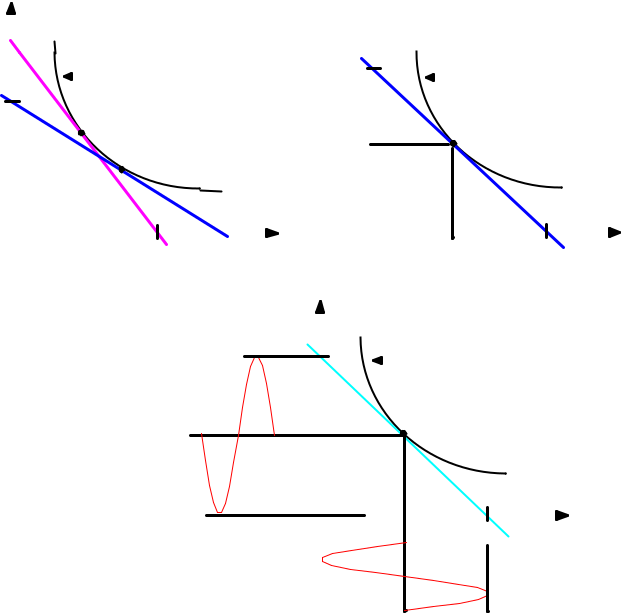
\includegraphics[width=0.45\textwidth]{./media/image8.png}
	\end{subfigure}
~
\end{figure}


%%%%%%%%%%%%%%%%%%%% Figure/Image No: 5 Ends here %%%%%%%%%%%%%%%%%%%%

\par


\vspace{\baselineskip}
\begin{adjustwidth}{3.53in}{0.0in}
\textit{\textsubscript{V \tabto{3.64in} = \tabto{3.72in} }\textsuperscript{V}}{\fontsize{3pt}{3.6pt}\selectfont C C\par}\par

\end{adjustwidth}

\begin{adjustwidth}{3.57in}{0.0in}
{\fontsize{3pt}{3.6pt}\selectfont C EQ\par}\par

\end{adjustwidth}

\par 
 \begin{tikzpicture}

\draw (3.72in,0.03in) -- (3.92in,0.03in); 

\end{tikzpicture}
\begin{adjustwidth}{3.79in}{0.0in}
{\fontsize{4pt}{4.8pt}\selectfont \textit{2}\par}\par

\end{adjustwidth}

\begin{adjustwidth}{3.44in}{0.0in}
{\fontsize{6pt}{7.2pt}\selectfont (c)\par}\par

\end{adjustwidth}


\vspace{\baselineskip}
{\fontsize{9pt}{10.8pt}\selectfont \ \ \ \ \ \ \ \ \ \ \ \ \ \ \ \ \ \ \ \ \ \ \  (a) Distintos puntos Q. (b) Punto Q para máxima excursión simétrica.\par}\par


\vspace{\baselineskip}
\begin{adjustwidth}{0.86in}{0.0in}
(c) Excursión de la corriente y el voltaje.\par

\end{adjustwidth}


\vspace{\baselineskip}
\begin{adjustwidth}{1.07in}{0.0in}
Para valores arbitrarios I\textsubscript{CMax} y V\textsubscript{CEMax}, el punto Q estará dado por la\par

\end{adjustwidth}

\begin{adjustwidth}{0.86in}{0.0in}
tangente a la curva P\textsubscript{CEMax}, en las coordenadas I\textsubscript{CQ}\ =  \uline{\textsuperscript{ICMax}}\  y V\textsubscript{CEQ} =\par

\end{adjustwidth}

\begin{adjustwidth}{4.68in}{0.0in}
2\par

\end{adjustwidth}

\begin{Center}
\uline{\textsuperscript{V}CEMax}\  de acuerdo a la Fig. \tabto{0.11in} 4b.\tab Se asume que la señal de entrada puede
\end{Center}\par

\begin{adjustwidth}{1.06in}{0.0in}
2\par

\end{adjustwidth}

\begin{adjustwidth}{0.86in}{0.88in}
\begin{justify}
{\fontsize{9pt}{10.8pt}\selectfont manejar el transistor entre el corte y la saturación, de esta forma para una variación en la corriente de base, se tiene la variación en la corriente de colector, y una variación en la potencia. La recta de carga de CA tiene la misma pendiente que la recta de carga de CC. En la Fig. 4c, se observan la onda de corriente i\textsubscript{C}\par}
\end{justify}\par

\end{adjustwidth}

\begin{adjustwidth}{0.86in}{0.0in}
y vCE: Note que la excursión será simétrica, así de acuerdo se tiene ICQ = \uline{\textsuperscript{V}CC}\par

\end{adjustwidth}

\begin{adjustwidth}{5.4in}{0.0in}
2R\textsubscript{L}\par

\end{adjustwidth}

\begin{adjustwidth}{0.86in}{0.0in}
y V\textsubscript{CEQ} = \uline{\textsuperscript{VCC}}\textsubscript{2} .\par

\end{adjustwidth}

\begin{adjustwidth}{1.07in}{0.88in}
{\fontsize{9pt}{10.8pt}\selectfont La Fig. 5, muestra las formas de onda a través del tiempo i\textsubscript{C}, v\textsubscript{CE}, p\textsubscript{CC}. La onda de potencia instantánea de la fuente p\textsubscript{CC}, estará dada por el pro\par}\par

\end{adjustwidth}

\begin{adjustwidth}{0.86in}{0.88in}
ducto V\textsubscript{CC}i\textsubscript{C} y tiene la misma forma que i\textsubscript{C}. P\textsubscript{CE} = i\textsubscript{c}v\textsubscript{CE}. Note que la forma de onda de P\textsubscript{CE} tiene una frecuencia el doble de las otras formas de onda.\par

\end{adjustwidth}


\vspace{\baselineskip}

\vspace{\baselineskip}

\vspace{\baselineskip}

\vspace{\baselineskip}
\begin{adjustwidth}{0.0in}{0.01in}
\begin{Center}
{\fontsize{8pt}{9.6pt}\selectfont 5\par}
\end{Center}\par

\end{adjustwidth}


\vspace{\baselineskip}

\vspace{\baselineskip}

\vspace{\baselineskip}

\vspace{\baselineskip}

\vspace{\baselineskip}


%%%%%%%%%%%%%%%%%%%% Figure/Image No: 6 starts here %%%%%%%%%%%%%%%%%%%%

\begin{figure}[H]
	\begin{Center}
		
\includegraphics[width=0.07in,height=0.08in]{./media/image9.png}
	\end{Center}
\end{figure}


%%%%%%%%%%%%%%%%%%%% Figure/Image No: 6 Ends here %%%%%%%%%%%%%%%%%%%%

\begin{adjustwidth}{2.29in}{0.0in}
{\fontsize{7pt}{8.4pt}\selectfont \textit{i}{\fontsize{5pt}{6.0pt}\selectfont \textit{C\  }\par}\par}\par

\end{adjustwidth}



%%%%%%%%%%%%%%%%%%%% Figure/Image No: 7 starts here %%%%%%%%%%%%%%%%%%%%

\begin{figure}[H]
\advance\leftskip 2.4in		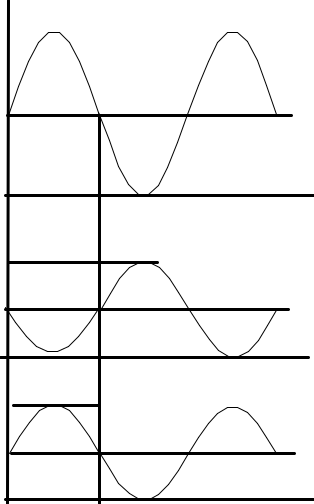
\includegraphics[width=1.45in,height=2.33in]{./media/image10.png}
\end{figure}


%%%%%%%%%%%%%%%%%%%% Figure/Image No: 7 Ends here %%%%%%%%%%%%%%%%%%%%

\par



%%%%%%%%%%%%%%%%%%%% Figure/Image No: 8 starts here %%%%%%%%%%%%%%%%%%%%

\begin{figure}[H]
	\begin{Center}
		
\includegraphics[width=1.07in,height=0.02in]{./media/image11.png}
	\end{Center}
\end{figure}


%%%%%%%%%%%%%%%%%%%% Figure/Image No: 8 Ends here %%%%%%%%%%%%%%%%%%%%

\begin{adjustwidth}{2.17in}{0.0in}
\textit{\textsuperscript{I}}{\fontsize{5pt}{6.0pt}\selectfont \textit{CMax }\par}\par

\end{adjustwidth}



%%%%%%%%%%%%%%%%%%%% Table No: 12 starts here %%%%%%%%%%%%%%%%%%%%


\begin{table}[H]
 			\centering
\begin{tabular}{p{0.02in}p{1.4in}p{-0.1in}p{0.02in}}
%row no:1
\multicolumn{1}{p{0.02in}}{\multirow{1}{*}{\begin{tabular}{p{0.02in}}\Centering \textit{\textsuperscript{I}}{\fontsize{5pt}{6.0pt}\selectfont \textit{CMax}}\\\end{tabular}}} & 
\multicolumn{1}{p{1.4in}}{\multirow{1}{*}{\begin{tabular}{p{1.4in}}\textit{\textsuperscript{I}}{\fontsize{5pt}{6.0pt}\selectfont \textit{CQ}}\\\end{tabular}}} & 
\multicolumn{1}{p{-0.1in}}{\multirow{1}{*}{\begin{tabular}{p{-0.1in}}{\fontsize{7pt}{8.4pt}\selectfont \textit{=}}\\\end{tabular}}} & 
\multicolumn{1}{p{0.02in}}{\Centering \textit{\textsuperscript{V}}{\fontsize{5pt}{6.0pt}\selectfont \textit{CC}}} \\
\hhline{~~~~}
%row no:2
\multicolumn{1}{p{0.02in}}{} & 
\multicolumn{1}{p{1.4in}}{} & 
\multicolumn{1}{p{-0.1in}}{} & 
\multicolumn{1}{p{0.02in}}{\multirow{1}{*}{\begin{tabular}{p{0.02in}}\Centering {\fontsize{5pt}{6.0pt}\selectfont \textit{2}{\fontsize{6pt}{7.2pt}\selectfont \textit{R}}}\\\end{tabular}}} \\ 

\hhline{~~~~}
%row no:3
\multicolumn{1}{p{0.02in}}{\multirow{1}{*}{\begin{tabular}{p{0.02in}}{\fontsize{5pt}{6.0pt}\selectfont \textit{2}}\\\end{tabular}}} & 
\multicolumn{1}{p{1.4in}}{} & 
\multicolumn{1}{p{-0.1in}}{} & 
\multicolumn{1}{p{0.02in}}{} \\
\hhline{~~~~}
%row no:4
\multicolumn{1}{p{0.02in}}{} & 
\multicolumn{1}{p{1.4in}}{} & 
\multicolumn{1}{p{-0.1in}}{} & 
\multicolumn{1}{p{0.02in}}{{\fontsize{5pt}{6.0pt}\selectfont \textit{L}}} \\
\hhline{~~~~}

\end{tabular}
 \end{table}


%%%%%%%%%%%%%%%%%%%% Table No: 12 ends here %%%%%%%%%%%%%%%%%%%%


\vspace{\baselineskip}
\begin{adjustwidth}{3.89in}{0.0in}
{\fontsize{6pt}{7.2pt}\selectfont \textit{ t}\par}\par

\end{adjustwidth}

\begin{enumerate}
	\item {\fontsize{5pt}{6.0pt}\selectfont \textit{CE}\par}
\end{enumerate}\par

\begin{adjustwidth}{2.12in}{0.0in}
\textit{\textsuperscript{V}}CE M ax\par

\end{adjustwidth}



%%%%%%%%%%%%%%%%%%%% Table No: 13 starts here %%%%%%%%%%%%%%%%%%%%


\begin{table}[H]
 			\centering
\begin{tabular}{p{0.77in}p{0.81in}p{-0.05in}}
%row no:1
\multicolumn{1}{p{0.77in}}{\multirow{1}{*}{\begin{tabular}{p{0.77in}}\textit{\textsuperscript{V}}{\fontsize{4pt}{4.8pt}\selectfont \textit{CE M ax}}\\\end{tabular}}} & 
\multicolumn{1}{p{0.81in}}{\multirow{1}{*}{\begin{tabular}{p{0.81in}}\textit{\textsuperscript{V}}{\fontsize{4pt}{4.8pt}\selectfont \textit{CEQ\ \  \textsuperscript{=}}}\\\end{tabular}}} & 
\multicolumn{1}{p{-0.05in}}{\Centering \textit{\textsuperscript{V}}{\fontsize{4pt}{4.8pt}\selectfont \textit{CC}}} \\
\hhline{~~~}
%row no:2
\multicolumn{1}{p{0.77in}}{} & 
\multicolumn{1}{p{0.81in}}{} & 
\multicolumn{1}{p{-0.05in}}{{\fontsize{5pt}{6.0pt}\selectfont \textit{2}}} \\
\hhline{~~~}

\end{tabular}
 \end{table}


%%%%%%%%%%%%%%%%%%%% Table No: 13 ends here %%%%%%%%%%%%%%%%%%%%

\par 
 \begin{tikzpicture}

\draw (2.16in,0.02in) -- (2.38in,0.02in); 

\draw (4.12in,0.09in) -- (4.34in,0.09in); 

\end{tikzpicture}
\begin{adjustwidth}{2.25in}{0.0in}
{\fontsize{5pt}{6.0pt}\selectfont \textit{2}\par}\par

\end{adjustwidth}


\vspace{\baselineskip}
\begin{adjustwidth}{3.86in}{0.0in}
{\fontsize{6pt}{7.2pt}\selectfont \textit{ t}\par}\par

\end{adjustwidth}

\begin{enumerate}
	\item {\fontsize{4pt}{4.8pt}\selectfont \textit{CC}\par}
\end{enumerate}\par


\vspace{\baselineskip}
\begin{adjustwidth}{3.82in}{0.0in}
{\fontsize{6pt}{7.2pt}\selectfont \textit{P \tabto{3.97in} =V \tabto{4.19in} I}\par}\par

\end{adjustwidth}

\begin{adjustwidth}{3.88in}{0.0in}
{\fontsize{4pt}{4.8pt}\selectfont \textit{CC \tabto{4.06in} CC \tabto{4.18in} }{\fontsize{5pt}{6.0pt}\selectfont \textit{CQ}\par}\par}\par

\end{adjustwidth}


\vspace{\baselineskip}
\begin{adjustwidth}{3.89in}{0.0in}
{\fontsize{6pt}{7.2pt}\selectfont \textit{ t}\par}\par

\end{adjustwidth}


\vspace{\baselineskip}
\begin{adjustwidth}{0.0in}{0.01in}
\begin{Center}
Figure 5: Curvas de i\textsubscript{C}, v\textsubscript{CE} y p\textsubscript{CC}.
\end{Center}\par

\end{adjustwidth}


\vspace{\baselineskip}

\vspace{\baselineskip}
\begin{adjustwidth}{0.86in}{0.0in}
\textcolor[HTML]{5C2D91}{4.1. Determinación de la Eficiencia}\par

\end{adjustwidth}


\vspace{\baselineskip}
\begin{adjustwidth}{0.86in}{0.0in}
La potencia en la carga será:\par

\end{adjustwidth}


\vspace{\baselineskip}


%%%%%%%%%%%%%%%%%%%% Table No: 14 starts here %%%%%%%%%%%%%%%%%%%%


\begin{table}[H]
 			\centering
\begin{tabular}{p{1.55in}p{0.88in}}
%row no:1
\multicolumn{1}{p{1.55in}}{\textsuperscript{P}{\fontsize{7pt}{8.4pt}\selectfont L \textsuperscript{=} \textsuperscript{I}Crms\textsuperscript{2R}L}} & 
\multicolumn{1}{p{0.88in}}{(11)} \\
\hhline{~~}

\end{tabular}
 \end{table}


%%%%%%%%%%%%%%%%%%%% Table No: 14 ends here %%%%%%%%%%%%%%%%%%%%

\begin{adjustwidth}{0.86in}{0.88in}
\begin{justify}
Luego de acuerdo a (9) o (10), considerando que la corriente tiene componente continua y alterna, se tiene:
\end{justify}\par

\end{adjustwidth}


\vspace{\baselineskip}


%%%%%%%%%%%%%%%%%%%% Table No: 15 starts here %%%%%%%%%%%%%%%%%%%%


{
\scriptsize
\setlength\extrarowheight{3pt}
\begin{longtable}{p{0.74in}p{0.09in}p{0.06in}p{-0.08in}p{-0.06in}p{-0.1in}p{-0.14in}p{-0.13in}p{-0.17in}p{-0.09in}p{-0.13in}p{-0.14in}p{-0.17in}p{-0.12in}p{-0.18in}p{-0.06in}p{-0.08in}p{-0.16in}p{-0.17in}p{-0.16in}p{0.02in}p{0.04in}p{-0.1in}p{0.02in}p{-0.03in}p{0.2in}p{0.26in}}

\endfirsthead
\multicolumn{27}{c}{\textit{continued from previous page}}\hline
\endhead\hline
\multicolumn{27}{r}{\textit{continued on next page}} \\
\endfoot
\hline 
\endlastfoot%row no:1
\multicolumn{1}{p{0.74in}}{} & 
\multicolumn{1}{p{0.09in}}{} & 
\multicolumn{1}{p{0.06in}}{} & 
\multicolumn{1}{p{-0.08in}}{} & 
\multicolumn{1}{p{-0.06in}}{} & 
\multicolumn{1}{p{-0.1in}}{} & 
\multicolumn{1}{p{-0.14in}}{} & 
\multicolumn{1}{p{-0.13in}}{} & 
\multicolumn{1}{p{-0.17in}}{} & 
\multicolumn{1}{p{-0.09in}}{} & 
\multicolumn{1}{p{-0.13in}}{} & 
\multicolumn{1}{p{-0.14in}}{} & 
\multicolumn{1}{p{-0.17in}}{} & 
\multicolumn{1}{p{-0.12in}}{\multirow{1}{*}{\begin{tabular}{p{-0.12in}}{\fontsize{7pt}{8.4pt}\selectfont 2}\\\end{tabular}}} & 
\multicolumn{1}{p{-0.18in}}{} & 
\multicolumn{1}{p{-0.06in}}{} & 
\multicolumn{1}{p{-0.08in}}{} & 
\multicolumn{1}{p{-0.16in}}{} & 
\multicolumn{1}{p{-0.17in}}{} & 
\multicolumn{1}{p{-0.16in}}{} & 
\multicolumn{1}{p{0.02in}}{} & 
\multicolumn{1}{p{0.04in}}{} & 
\multicolumn{1}{p{-0.1in}}{} & 
\multicolumn{1}{p{0.02in}}{} & 
\multicolumn{1}{p{-0.03in}}{} & 
\multicolumn{1}{p{0.2in}}{} & 
\multicolumn{1}{p{0.26in}}{} \\
\hhline{~~~~~~~~~~~~~~~~~~~~~~~~~~~}
%row no:2
\multicolumn{1}{p{0.74in}}{} & 
\multicolumn{1}{p{0.09in}}{} & 
\multicolumn{1}{p{0.06in}}{} & 
\multicolumn{1}{p{-0.08in}}{} & 
\multicolumn{6}{p{-0.06in}}{\multirow{1}{*}{\begin{tabular}{p{-0.06in}}\textsuperscript{I}{\fontsize{6pt}{7.2pt}\selectfont CQ}\\\end{tabular}}} & 
\multicolumn{1}{p{-0.13in}}{\multirow{1}{*}{\begin{tabular}{p{-0.13in}}{\fontsize{7pt}{8.4pt}\selectfont 2}\\\end{tabular}}} & 
\multicolumn{1}{p{-0.14in}}{} & 
\multicolumn{1}{p{-0.17in}}{} & 
\multicolumn{1}{p{-0.12in}}{} & 
\multicolumn{1}{p{-0.18in}}{} & 
\multicolumn{1}{p{-0.06in}}{} & 
\multicolumn{1}{p{-0.08in}}{} & 
\multicolumn{1}{p{-0.16in}}{} & 
\multicolumn{1}{p{-0.17in}}{} & 
\multicolumn{1}{p{-0.16in}}{} & 
\multicolumn{1}{p{0.02in}}{} & 
\multicolumn{1}{p{0.04in}}{} & 
\multicolumn{1}{p{-0.1in}}{} & 
\multicolumn{1}{p{0.02in}}{} & 
\multicolumn{1}{p{-0.03in}}{} & 
\multicolumn{1}{p{0.2in}}{} & 
\multicolumn{1}{p{0.26in}}{} \\
\hhline{~~~~~~~~~~~~~~~~~~~~~~~~~~~}
%row no:3
\multicolumn{1}{p{0.74in}}{} & 
\multicolumn{1}{p{0.09in}}{} & 
\multicolumn{1}{p{0.06in}}{} & 
\multicolumn{1}{p{-0.08in}}{} & 
\multicolumn{6}{p{-0.06in}}{} & 
\multicolumn{1}{p{-0.13in}}{} & 
\multicolumn{1}{p{-0.14in}}{} & 
\multicolumn{1}{p{-0.17in}}{} & 
\multicolumn{1}{p{-0.12in}}{} & 
\multicolumn{1}{p{-0.18in}}{} & 
\multicolumn{1}{p{-0.06in}}{} & 
\multicolumn{1}{p{-0.08in}}{} & 
\multicolumn{1}{p{-0.16in}}{} & 
\multicolumn{1}{p{-0.17in}}{} & 
\multicolumn{1}{p{-0.16in}}{} & 
\multicolumn{1}{p{0.02in}}{} & 
\multicolumn{1}{p{0.04in}}{} & 
\multicolumn{1}{p{-0.1in}}{} & 
\multicolumn{1}{p{0.02in}}{} & 
\multicolumn{1}{p{-0.03in}}{} & 
\multicolumn{1}{p{0.2in}}{} & 
\multicolumn{1}{p{0.26in}}{} \\
\hhline{~~~~~~~~~~~~~~~~~~~~~~~~~~~}
%row no:4
\multicolumn{1}{p{0.74in}}{} & 
\multicolumn{1}{p{0.09in}}{\multirow{1}{*}{\begin{tabular}{p{0.09in}}4\\\end{tabular}}} & 
\multicolumn{1}{p{0.06in}}{} & 
\multicolumn{1}{p{-0.08in}}{} & 
\multicolumn{6}{p{-0.06in}}{} & 
\multicolumn{3}{p{0.39in}}{\multirow{1}{*}{\begin{tabular}{p{0.39in}}5\\\end{tabular}}} & 
\multicolumn{1}{p{-0.12in}}{} & 
\multicolumn{1}{p{-0.18in}}{} & 
\multicolumn{1}{p{-0.06in}}{} & 
\multicolumn{1}{p{-0.08in}}{} & 
\multicolumn{1}{p{-0.16in}}{} & 
\multicolumn{1}{p{-0.17in}}{} & 
\multicolumn{1}{p{-0.16in}}{} & 
\multicolumn{1}{p{0.02in}}{} & 
\multicolumn{1}{p{0.04in}}{} & 
\multicolumn{1}{p{-0.1in}}{} & 
\multicolumn{1}{p{0.02in}}{} & 
\multicolumn{1}{p{-0.03in}}{} & 
\multicolumn{1}{p{0.2in}}{} & 
\multicolumn{1}{p{0.26in}}{} \\
\hhline{~~~~~~~~~~~~~~~~~~~~~~~~~~~}
%row no:5
\multicolumn{1}{p{0.74in}}{} & 
\multicolumn{1}{p{0.09in}}{} & 
\multicolumn{1}{p{0.06in}}{} & 
\multicolumn{1}{p{-0.08in}}{} & 
\multicolumn{1}{p{-0.06in}}{} & 
\multicolumn{1}{p{-0.1in}}{} & 
\multicolumn{1}{p{-0.14in}}{} & 
\multicolumn{1}{p{-0.13in}}{} & 
\multicolumn{1}{p{-0.17in}}{} & 
\multicolumn{1}{p{-0.09in}}{} & 
\multicolumn{3}{p{0.39in}}{} & 
\multicolumn{1}{p{-0.12in}}{} & 
\multicolumn{1}{p{-0.18in}}{} & 
\multicolumn{1}{p{-0.06in}}{} & 
\multicolumn{1}{p{-0.08in}}{} & 
\multicolumn{1}{p{-0.16in}}{} & 
\multicolumn{1}{p{-0.17in}}{} & 
\multicolumn{1}{p{-0.16in}}{} & 
\multicolumn{1}{p{0.02in}}{} & 
\multicolumn{1}{p{0.04in}}{} & 
\multicolumn{1}{p{-0.1in}}{} & 
\multicolumn{1}{p{0.02in}}{} & 
\multicolumn{1}{p{-0.03in}}{\multirow{1}{*}{\begin{tabular}{p{-0.03in}}{\fontsize{3pt}{3.6pt}\selectfont 2}\\\end{tabular}}} & 
\multicolumn{1}{p{0.2in}}{} & 
\multicolumn{1}{p{0.26in}}{} \\
\hhline{~~~~~~~~~~~~~~~~~~~~~~~~~~~}
%row no:6
\multicolumn{1}{p{0.74in}}{\multirow{1}{*}{\begin{tabular}{p{0.74in}}P\textsubscript{L}\  =\\\end{tabular}}} & 
\multicolumn{1}{p{0.09in}}{} & 
\multicolumn{1}{p{0.06in}}{} & 
\multicolumn{7}{p{-0.08in}}{\multirow{1}{*}{\begin{tabular}{p{-0.08in}}+\ \  p\textsubscript{2}\\\end{tabular}}} & 
\multicolumn{3}{p{0.39in}}{} & 
\multicolumn{1}{p{-0.12in}}{} & 
\multicolumn{1}{p{-0.18in}}{} & 
\multicolumn{1}{p{-0.06in}}{} & 
\multicolumn{1}{p{-0.08in}}{} & 
\multicolumn{1}{p{-0.16in}}{} & 
\multicolumn{1}{p{-0.17in}}{} & 
\multicolumn{1}{p{-0.16in}}{} & 
\multicolumn{1}{p{0.02in}}{} & 
\multicolumn{1}{p{0.04in}}{} & 
\multicolumn{1}{p{-0.1in}}{} & 
\multicolumn{1}{p{0.02in}}{} & 
\multicolumn{1}{p{-0.03in}}{} & 
\multicolumn{1}{p{0.2in}}{} & 
\multicolumn{1}{p{0.26in}}{} \\
\hhline{~~~~~~~~~~~~~~~~~~~~~~~~~~~}
%row no:7
\multicolumn{1}{p{0.74in}}{} & 
\multicolumn{2}{p{0.09in}}{\textsuperscript{2s}\textsubscript{ICQ}{\fontsize{7pt}{8.4pt}\selectfont 2}} & 
\multicolumn{7}{p{-0.08in}}{} & 
\multicolumn{1}{p{-0.13in}}{} & 
\multicolumn{6}{p{-0.14in}}{\textsuperscript{3} R\textsubscript{L}} & 
\multicolumn{1}{p{-0.16in}}{} & 
\multicolumn{1}{p{-0.17in}}{} & 
\multicolumn{1}{p{-0.16in}}{} & 
\multicolumn{1}{p{0.02in}}{} & 
\multicolumn{1}{p{0.04in}}{} & 
\multicolumn{1}{p{-0.1in}}{\multirow{1}{*}{\begin{tabular}{p{-0.1in}}\end{tabular}}} & 
\multicolumn{1}{p{0.02in}}{} & 
\multicolumn{1}{p{-0.03in}}{\multirow{1}{*}{\begin{tabular}{p{-0.03in}}\end{tabular}}} & 
\multicolumn{1}{p{0.2in}}{} & 
\multicolumn{1}{p{0.26in}}{} \\
\hhline{~~~~~~~~~~~~~~~~~~~~~~~~~~~}
%row no:8
\multicolumn{1}{p{0.74in}}{} & 
\multicolumn{1}{p{0.09in}}{} & 
\multicolumn{1}{p{0.06in}}{} & 
\multicolumn{7}{p{-0.08in}}{\multirow{1}{*}{\begin{tabular}{p{-0.08in}}\Centering I\textsubscript{CQ}\textsuperscript{2}\\\end{tabular}}} & 
\multicolumn{1}{p{-0.13in}}{} & 
\multicolumn{1}{p{-0.14in}}{} & 
\multicolumn{1}{p{-0.17in}}{} & 
\multicolumn{1}{p{-0.12in}}{} & 
\multicolumn{3}{p{-0.18in}}{\multirow{1}{*}{\begin{tabular}{p{-0.18in}}\textsuperscript{V}{\fontsize{6pt}{7.2pt}\selectfont CC}\\\end{tabular}}} & 
\multicolumn{1}{p{-0.16in}}{} & 
\multicolumn{1}{p{-0.17in}}{} & 
\multicolumn{1}{p{-0.16in}}{} & 
\multicolumn{1}{p{0.02in}}{\multirow{1}{*}{\begin{tabular}{p{0.02in}}{\fontsize{7pt}{8.4pt}\selectfont 2}\\\end{tabular}}} & 
\multicolumn{1}{p{0.04in}}{} & 
\multicolumn{1}{p{-0.1in}}{} & 
\multicolumn{1}{p{0.02in}}{\textsuperscript{V}{\fontsize{3pt}{3.6pt}\selectfont CC}} & 
\multicolumn{1}{p{-0.03in}}{} & 
\multicolumn{1}{p{0.2in}}{} & 
\multicolumn{1}{p{0.26in}}{} \\
\hhline{~~~~~~~~~~~~~~~~~~~~~~~~~~~}
%row no:9
\multicolumn{1}{p{0.74in}}{} & 
\multicolumn{1}{p{0.09in}}{} & 
\multicolumn{1}{p{0.06in}}{} & 
\multicolumn{7}{p{-0.08in}}{} & 
\multicolumn{1}{p{-0.13in}}{} & 
\multicolumn{1}{p{-0.14in}}{} & 
\multicolumn{1}{p{-0.17in}}{} & 
\multicolumn{1}{p{-0.12in}}{} & 
\multicolumn{3}{p{-0.18in}}{} & 
\multicolumn{1}{p{-0.16in}}{} & 
\multicolumn{1}{p{-0.17in}}{} & 
\multicolumn{1}{p{-0.16in}}{} & 
\multicolumn{1}{p{0.02in}}{} & 
\multicolumn{1}{p{0.04in}}{} & 
\multicolumn{1}{p{-0.1in}}{} & 
\multicolumn{1}{p{0.02in}}{{\fontsize{5pt}{6.0pt}\selectfont 2R\textsubscript{L}}} & 
\multicolumn{1}{p{-0.03in}}{} & 
\multicolumn{1}{p{0.2in}}{} & 
\multicolumn{1}{p{0.26in}}{} \\
\hhline{~~~~~~~~~~~~~~~~~~~~~~~~~~~}
%row no:10
\multicolumn{1}{p{0.74in}}{\multirow{1}{*}{\begin{tabular}{p{0.74in}}=\\\end{tabular}}} & 
\multicolumn{3}{p{0.09in}}{\multirow{1}{*}{\begin{tabular}{p{0.09in}}I\textsubscript{CQ}\textsuperscript{2}R\textsubscript{L} +\\\end{tabular}}} & 
\multicolumn{2}{p{-0.06in}}{} & 
\multicolumn{8}{p{-0.14in}}{\multirow{1}{*}{\begin{tabular}{p{-0.14in}}R\textsubscript{L} =\\\end{tabular}}} & 
\multicolumn{1}{p{-0.18in}}{} & 
\multicolumn{1}{p{-0.06in}}{} & 
\multicolumn{1}{p{-0.08in}}{} & 
\multicolumn{3}{p{0.7in}}{\multirow{1}{*}{\begin{tabular}{p{0.7in}}\end{tabular}}} & 
\multicolumn{2}{p{0.02in}}{\multirow{1}{*}{\begin{tabular}{p{0.02in}}R\textsubscript{L} +\\\end{tabular}}} & 
\multicolumn{1}{p{-0.1in}}{} & 
\multicolumn{1}{p{0.02in}}{} & 
\multicolumn{1}{p{-0.03in}}{} & 
\multicolumn{1}{p{0.2in}}{\multirow{1}{*}{\begin{tabular}{p{0.2in}}R\textsubscript{L}\\\end{tabular}}} & 
\multicolumn{1}{p{0.26in}}{\multirow{1}{*}{\begin{tabular}{p{0.26in}}(12)\\\end{tabular}}} \\ 

\hhline{~~~~~~~~~~~~~~~~~~~~~~~~~~~}
%row no:11
\multicolumn{1}{p{0.74in}}{} & 
\multicolumn{3}{p{0.09in}}{} & 
\multicolumn{2}{p{-0.06in}}{2} & 
\multicolumn{8}{p{-0.14in}}{} & 
\multicolumn{1}{p{-0.18in}}{} & 
\multicolumn{2}{p{-0.06in}}{2R\textsubscript{L}} & 
\multicolumn{3}{p{0.7in}}{} & 
\multicolumn{2}{p{0.02in}}{} & 
\multicolumn{1}{p{-0.1in}}{} & 
\multicolumn{1}{p{0.02in}}{2} & 
\multicolumn{1}{p{-0.03in}}{} & 
\multicolumn{1}{p{0.2in}}{} & 
\multicolumn{1}{p{0.26in}}{} \\
\hhline{~~~~~~~~~~~~~~~~~~~~~~~~~~~}
%row no:12
\multicolumn{1}{p{0.74in}}{Entonces} & 
\multicolumn{1}{p{0.09in}}{} & 
\multicolumn{1}{p{0.06in}}{} & 
\multicolumn{1}{p{-0.08in}}{} & 
\multicolumn{1}{p{-0.06in}}{} & 
\multicolumn{1}{p{-0.1in}}{} & 
\multicolumn{1}{p{-0.14in}}{} & 
\multicolumn{1}{p{-0.13in}}{} & 
\multicolumn{1}{p{-0.17in}}{} & 
\multicolumn{1}{p{-0.09in}}{} & 
\multicolumn{1}{p{-0.13in}}{} & 
\multicolumn{1}{p{-0.14in}}{} & 
\multicolumn{1}{p{-0.17in}}{} & 
\multicolumn{1}{p{-0.12in}}{} & 
\multicolumn{1}{p{-0.18in}}{} & 
\multicolumn{1}{p{-0.06in}}{} & 
\multicolumn{1}{p{-0.08in}}{} & 
\multicolumn{1}{p{-0.16in}}{} & 
\multicolumn{1}{p{-0.17in}}{} & 
\multicolumn{1}{p{-0.16in}}{} & 
\multicolumn{1}{p{0.02in}}{} & 
\multicolumn{1}{p{0.04in}}{} & 
\multicolumn{1}{p{-0.1in}}{} & 
\multicolumn{1}{p{0.02in}}{} & 
\multicolumn{1}{p{-0.03in}}{} & 
\multicolumn{1}{p{0.2in}}{} & 
\multicolumn{1}{p{0.26in}}{} \\
\hhline{~~~~~~~~~~~~~~~~~~~~~~~~~~~}
%row no:13
\multicolumn{1}{p{0.74in}}{} & 
\multicolumn{1}{p{0.09in}}{} & 
\multicolumn{1}{p{0.06in}}{} & 
\multicolumn{1}{p{-0.08in}}{} & 
\multicolumn{1}{p{-0.06in}}{} & 
\multicolumn{1}{p{-0.1in}}{} & 
\multicolumn{1}{p{-0.14in}}{} & 
\multicolumn{1}{p{-0.13in}}{} & 
\multicolumn{1}{p{-0.17in}}{} & 
\multicolumn{1}{p{-0.09in}}{} & 
\multicolumn{1}{p{-0.13in}}{} & 
\multicolumn{1}{p{-0.14in}}{} & 
\multicolumn{2}{p{0.7in}}{V} & 
\multicolumn{2}{p{0.39in}}{{\fontsize{7pt}{8.4pt}\selectfont 2}} & 
\multicolumn{1}{p{-0.08in}}{} & 
\multicolumn{1}{p{-0.16in}}{} & 
\multicolumn{4}{p{-0.17in}}{V \textsuperscript{2}} & 
\multicolumn{1}{p{-0.1in}}{} & 
\multicolumn{1}{p{0.02in}}{} & 
\multicolumn{1}{p{-0.03in}}{} & 
\multicolumn{1}{p{0.2in}}{} & 
\multicolumn{1}{p{0.26in}}{} \\
\hhline{~~~~~~~~~~~~~~~~~~~~~~~~~~~}
%row no:14
\multicolumn{1}{p{0.74in}}{} & 
\multicolumn{2}{p{0.09in}}{\multirow{1}{*}{\begin{tabular}{p{0.09in}}{\fontsize{6pt}{7.2pt}\selectfont P\textsubscript{L}}\\\end{tabular}}} & 
\multicolumn{2}{p{-0.08in}}{\multirow{1}{*}{\begin{tabular}{p{-0.08in}}{\fontsize{7pt}{8.4pt}\selectfont =}\\\end{tabular}}} & 
\multicolumn{1}{p{-0.1in}}{} & 
\multicolumn{1}{p{-0.14in}}{} & 
\multicolumn{1}{p{-0.13in}}{} & 
\multicolumn{1}{p{-0.17in}}{} & 
\multicolumn{1}{p{-0.09in}}{} & 
\multicolumn{1}{p{-0.13in}}{} & 
\multicolumn{1}{p{-0.14in}}{} & 
\multicolumn{1}{p{-0.17in}}{} & 
\multicolumn{3}{p{-0.12in}}{{\fontsize{3pt}{3.6pt}\selectfont CC}} & 
\multicolumn{2}{p{0.23in}}{\multirow{1}{*}{\begin{tabular}{p{0.23in}}{\fontsize{7pt}{8.4pt}\selectfont +}\\\end{tabular}}} & 
\multicolumn{1}{p{-0.17in}}{} & 
\multicolumn{1}{p{-0.16in}}{} & 
\multicolumn{1}{p{0.02in}}{{\fontsize{3pt}{3.6pt}\selectfont CC}} & 
\multicolumn{1}{p{0.04in}}{} & 
\multicolumn{1}{p{-0.1in}}{} & 
\multicolumn{1}{p{0.02in}}{} & 
\multicolumn{1}{p{-0.03in}}{} & 
\multicolumn{1}{p{0.2in}}{} & 
\multicolumn{1}{p{0.26in}}{\multirow{1}{*}{\begin{tabular}{p{0.26in}}{\fontsize{7pt}{8.4pt}\selectfont (13)}\\\end{tabular}}} \\ 

\hhline{~~~~~~~~~~~~~~~~~~~~~~~~~~~}
%row no:15
\multicolumn{1}{p{0.74in}}{} & 
\multicolumn{2}{p{0.09in}}{} & 
\multicolumn{2}{p{-0.08in}}{} & 
\multicolumn{1}{p{-0.1in}}{} & 
\multicolumn{1}{p{-0.14in}}{} & 
\multicolumn{1}{p{-0.13in}}{} & 
\multicolumn{1}{p{-0.17in}}{} & 
\multicolumn{1}{p{-0.09in}}{} & 
\multicolumn{1}{p{-0.13in}}{} & 
\multicolumn{1}{p{-0.14in}}{} & 
\multicolumn{1}{p{-0.17in}}{} & 
\multicolumn{3}{p{-0.12in}}{} & 
\multicolumn{2}{p{0.23in}}{} & 
\multicolumn{1}{p{-0.17in}}{} & 
\multicolumn{3}{p{-0.16in}}{\multirow{1}{*}{\begin{tabular}{p{-0.16in}}8R\textsubscript{L}\\\end{tabular}}} & 
\multicolumn{1}{p{-0.1in}}{} & 
\multicolumn{1}{p{0.02in}}{} & 
\multicolumn{1}{p{-0.03in}}{} & 
\multicolumn{1}{p{0.2in}}{} & 
\multicolumn{1}{p{0.26in}}{} \\
\hhline{~~~~~~~~~~~~~~~~~~~~~~~~~~~}
%row no:16
\multicolumn{1}{p{0.74in}}{} & 
\multicolumn{1}{p{0.09in}}{} & 
\multicolumn{1}{p{0.06in}}{} & 
\multicolumn{1}{p{-0.08in}}{} & 
\multicolumn{1}{p{-0.06in}}{} & 
\multicolumn{1}{p{-0.1in}}{} & 
\multicolumn{1}{p{-0.14in}}{} & 
\multicolumn{1}{p{-0.13in}}{} & 
\multicolumn{1}{p{-0.17in}}{} & 
\multicolumn{1}{p{-0.09in}}{} & 
\multicolumn{1}{p{-0.13in}}{} & 
\multicolumn{1}{p{-0.14in}}{} & 
\multicolumn{5}{p{-0.17in}}{4R\textsubscript{L}} & 
\multicolumn{1}{p{-0.16in}}{} & 
\multicolumn{1}{p{-0.17in}}{} & 
\multicolumn{3}{p{-0.16in}}{} & 
\multicolumn{1}{p{-0.1in}}{} & 
\multicolumn{1}{p{0.02in}}{} & 
\multicolumn{1}{p{-0.03in}}{} & 
\multicolumn{1}{p{0.2in}}{} & 
\multicolumn{1}{p{0.26in}}{} \\
\hhline{~~~~~~~~~~~~~~~~~~~~~~~~~~~}
%row no:17
\multicolumn{1}{p{0.74in}}{} & 
\multicolumn{1}{p{0.09in}}{} & 
\multicolumn{1}{p{0.06in}}{} & 
\multicolumn{1}{p{-0.08in}}{} & 
\multicolumn{1}{p{-0.06in}}{} & 
\multicolumn{1}{p{-0.1in}}{} & 
\multicolumn{1}{p{-0.14in}}{} & 
\multicolumn{1}{p{-0.13in}}{} & 
\multicolumn{1}{p{-0.17in}}{} & 
\multicolumn{1}{p{-0.09in}}{} & 
\multicolumn{4}{p{-0.13in}}{"} & 
\multicolumn{1}{p{-0.18in}}{} & 
\multicolumn{1}{p{-0.06in}}{} & 
\multicolumn{1}{p{-0.08in}}{} & 
\multicolumn{1}{p{-0.16in}}{} & 
\multicolumn{1}{p{-0.17in}}{} & 
\multicolumn{1}{p{-0.16in}}{} & 
\multicolumn{1}{p{0.02in}}{"} & 
\multicolumn{1}{p{0.04in}}{} & 
\multicolumn{1}{p{-0.1in}}{} & 
\multicolumn{1}{p{0.02in}}{} & 
\multicolumn{1}{p{-0.03in}}{} & 
\multicolumn{1}{p{0.2in}}{} & 
\multicolumn{1}{p{0.26in}}{} \\
\hhline{~~~~~~~~~~~~~~~~~~~~~~~~~~~}

\end{longtable}}

%%%%%%%%%%%%%%%%%%%% Table No: 15 ends here %%%%%%%%%%%%%%%%%%%%

\begin{adjustwidth}{3.14in}{0.0in}
\textsuperscript{P}{\fontsize{7pt}{8.4pt}\selectfont L(CC) \tabto{3.69in} \textsuperscript{P}{\fontsize{6pt}{7.2pt}\selectfont L(CA)\par}\par}\par

\end{adjustwidth}

\begin{adjustwidth}{1.07in}{0.0in}
Por otro lado, la potencia promedio entregada por la fuente será\par

\end{adjustwidth}


\vspace{\baselineskip}
\begin{adjustwidth}{3.68in}{0.0in}
V \textsuperscript{2}\par

\end{adjustwidth}

\begin{adjustwidth}{0.0in}{0.88in}
\begin{FlushRight}
{\fontsize{7pt}{8.4pt}\selectfont P\textsubscript{CC} = V\textsubscript{CC}I\textsubscript{CQ} = \tabto{0.22in} \textsuperscript{CC \tabto{1.85in} }{\fontsize{9pt}{10.8pt}\selectfont (14)\par}\par}
\end{FlushRight}\par

\end{adjustwidth}

\par 
 \begin{tikzpicture}

\draw (3.68in,0.03in) -- (3.94in,0.03in); 

\end{tikzpicture}
\begin{adjustwidth}{3.68in}{0.0in}
{\fontsize{8pt}{9.6pt}\selectfont 2R\textsubscript{L}\par}\par

\end{adjustwidth}


\vspace{\baselineskip}
\begin{adjustwidth}{0.0in}{0.01in}
\begin{Center}
{\fontsize{8pt}{9.6pt}\selectfont 6\par}
\end{Center}\par

\end{adjustwidth}


\vspace{\baselineskip}

\vspace{\baselineskip}

\vspace{\baselineskip}

\vspace{\baselineskip}

\vspace{\baselineskip}
\begin{adjustwidth}{1.07in}{0.0in}
Finalmente, la eficiencia estará dada por:\par

\end{adjustwidth}


\vspace{\baselineskip}


%%%%%%%%%%%%%%%%%%%% Table No: 16 starts here %%%%%%%%%%%%%%%%%%%%


\begin{table}[H]
 			\centering
\begin{tabular}{p{0.06in}p{-0.17in}p{0.01in}p{-0.17in}p{1.06in}p{0.87in}}
%row no:1
\multicolumn{1}{p{0.06in}}{} & 
\multicolumn{1}{p{-0.17in}}{} & 
\multicolumn{1}{p{0.01in}}{{\fontsize{7pt}{8.4pt}\selectfont V \textsuperscript{2}}} & 
\multicolumn{1}{p{-0.17in}}{} & 
\multicolumn{1}{p{1.06in}}{} & 
\multicolumn{1}{p{0.87in}}{} \\
\hhline{~~~~~~}
%row no:2
\multicolumn{1}{p{0.06in}}{} & 
\multicolumn{1}{p{-0.17in}}{} & 
\multicolumn{1}{p{0.01in}}{{\fontsize{2pt}{2.4pt}\selectfont CC}} & 
\multicolumn{1}{p{-0.17in}}{} & 
\multicolumn{1}{p{1.06in}}{} & 
\multicolumn{1}{p{0.87in}}{} \\
\hhline{~~~~~~}
%row no:3
\multicolumn{1}{p{0.06in}}{\multirow{1}{*}{\begin{tabular}{p{0.06in}}=\\\end{tabular}}} & 
\multicolumn{1}{p{-0.17in}}{} & 
\multicolumn{1}{p{0.01in}}{{\fontsize{6pt}{7.2pt}\selectfont 8R\textsubscript{L}}} & 
\multicolumn{1}{p{-0.17in}}{} & 
\multicolumn{1}{p{1.06in}}{\multirow{1}{*}{\begin{tabular}{p{1.06in}}= 0:25\\\end{tabular}}} & 
\multicolumn{1}{p{0.87in}}{\multirow{1}{*}{\begin{tabular}{p{0.87in}}(15)\\\end{tabular}}} \\ 

\hhline{~~~~~~}
%row no:4
\multicolumn{1}{p{0.06in}}{} & 
\multicolumn{1}{p{-0.17in}}{} & 
\multicolumn{1}{p{0.01in}}{\textsubscript{V}{\fontsize{3pt}{3.6pt}\selectfont  2}} & 
\multicolumn{1}{p{-0.17in}}{} & 
\multicolumn{1}{p{1.06in}}{} & 
\multicolumn{1}{p{0.87in}}{} \\
\hhline{~~~~~~}
%row no:5
\multicolumn{1}{p{0.06in}}{} & 
\multicolumn{1}{p{-0.17in}}{} & 
\multicolumn{1}{p{0.01in}}{{\fontsize{4pt}{4.8pt}\selectfont CC}} & 
\multicolumn{1}{p{-0.17in}}{} & 
\multicolumn{1}{p{1.06in}}{} & 
\multicolumn{1}{p{0.87in}}{} \\
\hhline{~~~~~~}

\end{tabular}
 \end{table}


%%%%%%%%%%%%%%%%%%%% Table No: 16 ends here %%%%%%%%%%%%%%%%%%%%

\begin{adjustwidth}{0.0in}{0.18in}
\begin{Center}
{\fontsize{6pt}{7.2pt}\selectfont 2R\textsubscript{L}\par}
\end{Center}\par

\end{adjustwidth}


\vspace{\baselineskip}
\begin{adjustwidth}{0.86in}{0.88in}
\begin{justify}
La eficiencia de este amplificador es baja, 25$\%$ , esto debido principalmente a que se mantiene una corriente de reposo en la carga, la cual no es usada (desperdiciada).
\end{justify}\par

\end{adjustwidth}


\vspace{\baselineskip}
\begin{adjustwidth}{1.07in}{0.0in}
La potencia disipada en el transistor será:\par

\end{adjustwidth}


\vspace{\baselineskip}


%%%%%%%%%%%%%%%%%%%% Table No: 17 starts here %%%%%%%%%%%%%%%%%%%%


\begin{table}[H]
 			\centering
\begin{tabular}{p{0.38in}p{-0.12in}p{0.06in}p{0.09in}p{-0.18in}p{0.06in}p{-0.01in}p{0.06in}p{0.12in}p{0.06in}p{-0.01in}p{0.06in}p{0.69in}}
%row no:1
\multicolumn{1}{p{0.38in}}{P\textsubscript{CE}\  =} & 
\multicolumn{5}{p{0.72in}}{P\textsubscript{CC}\ \  P\textsubscript{L}} & 
\multicolumn{1}{p{-0.01in}}{} & 
\multicolumn{1}{p{0.06in}}{} & 
\multicolumn{1}{p{0.12in}}{} & 
\multicolumn{1}{p{0.06in}}{} & 
\multicolumn{1}{p{-0.01in}}{} & 
\multicolumn{1}{p{0.06in}}{} & 
\multicolumn{1}{p{0.69in}}{} \\
\hhline{~~~~~~~~~~~~~}
%row no:2
\multicolumn{1}{p{0.38in}}{} & 
\multicolumn{1}{p{-0.12in}}{} & 
\multicolumn{1}{p{0.06in}}{\textsubscript{V}{\fontsize{6pt}{7.2pt}\selectfont  2}} & 
\multicolumn{1}{p{0.09in}}{\multirow{1}{*}{\begin{tabular}{p{0.09in}}\end{tabular}}} & 
\multicolumn{2}{p{0.08in}}{\textsubscript{V}{\fontsize{6pt}{7.2pt}\selectfont  2}} & 
\multicolumn{1}{p{-0.01in}}{} & 
\multicolumn{1}{p{0.06in}}{\textsubscript{V}{\fontsize{6pt}{7.2pt}\selectfont  2}} & 
\multicolumn{1}{p{0.12in}}{\multirow{1}{*}{\begin{tabular}{p{0.12in}}\textsubscript{=}\\\end{tabular}}} & 
\multicolumn{1}{p{0.06in}}{\textsubscript{V}{\fontsize{6pt}{7.2pt}\selectfont  2}} & 
\multicolumn{1}{p{-0.01in}}{} & 
\multicolumn{1}{p{0.06in}}{\textsubscript{V}{\fontsize{6pt}{7.2pt}\selectfont  2}} & 
\multicolumn{1}{p{0.69in}}{} \\
\hhline{~~~~~~~~~~~~~}
%row no:3
\multicolumn{1}{p{0.38in}}{\multirow{1}{*}{\begin{tabular}{p{0.38in}}=\\\end{tabular}}} & 
\multicolumn{1}{p{-0.12in}}{} & 
\multicolumn{1}{p{0.06in}}{{\fontsize{4pt}{4.8pt}\selectfont CC}} & 
\multicolumn{1}{p{0.09in}}{} & 
\multicolumn{1}{p{-0.18in}}{} & 
\multicolumn{1}{p{0.06in}}{{\fontsize{4pt}{4.8pt}\selectfont CC}} & 
\multicolumn{1}{p{-0.01in}}{\multirow{1}{*}{\begin{tabular}{p{-0.01in}}+\\\end{tabular}}} & 
\multicolumn{1}{p{0.06in}}{{\fontsize{4pt}{4.8pt}\selectfont CC}} & 
\multicolumn{1}{p{0.12in}}{} & 
\multicolumn{1}{p{0.06in}}{{\fontsize{4pt}{4.8pt}\selectfont CC}} & 
\multicolumn{1}{p{-0.01in}}{\multirow{1}{*}{\begin{tabular}{p{-0.01in}}\end{tabular}}} & 
\multicolumn{1}{p{0.06in}}{{\fontsize{4pt}{4.8pt}\selectfont CC}} & 
\multicolumn{1}{p{0.69in}}{\multirow{1}{*}{\begin{tabular}{p{0.69in}}(16)\\\end{tabular}}} \\ 

\hhline{~~~~~~~~~~~~~}
%row no:4
\multicolumn{1}{p{0.38in}}{} & 
\multicolumn{1}{p{-0.12in}}{} & 
\multicolumn{1}{p{0.06in}}{2R\textsubscript{L}} & 
\multicolumn{1}{p{0.09in}}{} & 
\multicolumn{1}{p{-0.18in}}{} & 
\multicolumn{1}{p{0.06in}}{4R\textsubscript{L}} & 
\multicolumn{1}{p{-0.01in}}{} & 
\multicolumn{1}{p{0.06in}}{8R\textsubscript{L}} & 
\multicolumn{1}{p{0.12in}}{} & 
\multicolumn{1}{p{0.06in}}{4R\textsubscript{L}} & 
\multicolumn{1}{p{-0.01in}}{} & 
\multicolumn{1}{p{0.06in}}{8R\textsubscript{L}} & 
\multicolumn{1}{p{0.69in}}{} \\
\hhline{~~~~~~~~~~~~~}

\end{tabular}
 \end{table}


%%%%%%%%%%%%%%%%%%%% Table No: 17 ends here %%%%%%%%%%%%%%%%%%%%


\vspace{\baselineskip}
\begin{adjustwidth}{0.86in}{0.0in}
\textcolor[HTML]{5C2D91}{4.2 \tabto{1.26in} Configuración emisor común con transformador de acoplo}\par

\end{adjustwidth}


\vspace{\baselineskip}
\begin{adjustwidth}{0.86in}{0.88in}
\begin{justify}
{\fontsize{9pt}{10.8pt}\selectfont Sea el circuito de la Fig. 6a. Una forma de mejorar la eficiencia del amplificador clase A es usar el acoplo de la carga mediante un transformador. ¿Cómo es eso?\par}
\end{justify}\par

\end{adjustwidth}


\vspace{\baselineskip}


%%%%%%%%%%%%%%%%%%%% Table No: 18 starts here %%%%%%%%%%%%%%%%%%%%


\begin{table}[H]
 			\centering
\begin{tabular}{p{0.06in}p{0.12in}p{0.3in}p{0.16in}p{-0.13in}}
%row no:1
\multicolumn{1}{p{0.06in}}{{\fontsize{6pt}{7.2pt}\selectfont \textit{V}{\fontsize{4pt}{4.8pt}\selectfont \textit{CC}}}} & 
\multicolumn{1}{p{0.12in}}{} & 
\multicolumn{1}{p{0.3in}}{} & 
\multicolumn{2}{p{0.23in}}{\textit{\textsuperscript{V}}{\fontsize{5pt}{6.0pt}\selectfont \textit{CC}}} \\
\hhline{~~~~~}
%row no:2
\multicolumn{1}{p{0.06in}}{{\fontsize{6pt}{7.2pt}\selectfont \textit{N}}} & 
\multicolumn{1}{p{0.12in}}{\multirow{1}{*}{\begin{tabular}{p{0.12in}}{\fontsize{6pt}{7.2pt}\selectfont \textit{N}}\\\end{tabular}}} & 
\multicolumn{1}{p{0.3in}}{{\fontsize{6pt}{7.2pt}\selectfont \textit{R\textsubscript{L}}}} & 
\multicolumn{1}{p{0.16in}}{\multirow{1}{*}{\begin{tabular}{p{0.16in}}{\fontsize{6pt}{7.2pt}\selectfont \textit{R}}\\\end{tabular}}} & 
\multicolumn{1}{p{-0.13in}}{{\fontsize{5pt}{6.0pt}\selectfont \textit{'}}} \\
\hhline{~~~~~}
%row no:3
\multicolumn{1}{p{0.06in}}{{\fontsize{1pt}{1.2pt}\selectfont \textit{p}}} & 
\multicolumn{1}{p{0.12in}}{} & 
\multicolumn{1}{p{0.3in}}{} & 
\multicolumn{1}{p{0.16in}}{} & 
\multicolumn{1}{p{-0.13in}}{\multirow{1}{*}{\begin{tabular}{p{-0.13in}}{\fontsize{5pt}{6.0pt}\selectfont \textit{L}}\\\end{tabular}}} \\ 

\hhline{~~~~~}
%row no:4
\multicolumn{1}{p{0.06in}}{} & 
\multicolumn{1}{p{0.12in}}{{\fontsize{5pt}{6.0pt}\selectfont \textit{s}}} & 
\multicolumn{1}{p{0.3in}}{} & 
\multicolumn{1}{p{0.16in}}{} & 
\multicolumn{1}{p{-0.13in}}{} \\
\hhline{~~~~~}

\end{tabular}
 \end{table}


%%%%%%%%%%%%%%%%%%%% Table No: 18 ends here %%%%%%%%%%%%%%%%%%%%



%%%%%%%%%%%%%%%%%%%% Figure/Image No: 9 starts here %%%%%%%%%%%%%%%%%%%%

\begin{figure}[H]
\advance\leftskip 2.03in		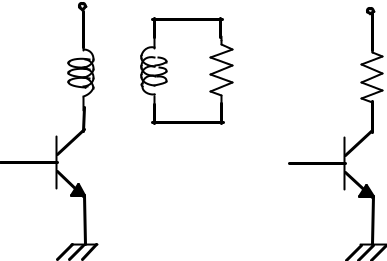
\includegraphics[width=1.79in,height=1.21in]{./media/image12.png}
\end{figure}


%%%%%%%%%%%%%%%%%%%% Figure/Image No: 9 Ends here %%%%%%%%%%%%%%%%%%%%

\par


\vspace{\baselineskip}
\begin{adjustwidth}{4.25in}{0.0in}
{\fontsize{5pt}{6.0pt}\selectfont \textit{2}\par}\par

\end{adjustwidth}

\begin{adjustwidth}{4.0in}{0.0in}
\textit{\textsubscript{' \tabto{4.17in} }\textsuperscript{N}}{\fontsize{3pt}{3.6pt}\selectfont \textit{p \tabto{4.32in} \textsubscript{R}}\par}\par

\end{adjustwidth}

\begin{adjustwidth}{3.93in}{0.0in}
\textit{\textsuperscript{R}}{\fontsize{4pt}{4.8pt}\selectfont \textit{L \tabto{4.07in} \textsuperscript{= }\textsubscript{Ns}2\ \ \  L}\par}\par

\end{adjustwidth}

\par 
 \begin{tikzpicture}

\draw (4.14in,0.15in) -- (4.3in,0.15in); 

\end{tikzpicture}

\vspace{\baselineskip}

\vspace{\baselineskip}
\begin{adjustwidth}{2.25in}{0.0in}
{\fontsize{6pt}{7.2pt}\selectfont (a ) \tabto{3.62in} \textsubscript{(b)}\par}\par

\end{adjustwidth}

\begin{adjustwidth}{0.0in}{0.01in}
\begin{Center}
(a) Amplificador acoplado por transformador. (b) Equivalente.
\end{Center}\par

\end{adjustwidth}


\vspace{\baselineskip}

\vspace{\baselineskip}
\begin{adjustwidth}{1.07in}{0.0in}
Para CC y CA se obtienen los circuitos equivalentes de la Fig .7.\par

\end{adjustwidth}



%%%%%%%%%%%%%%%%%%%% Figure/Image No: 10 starts here %%%%%%%%%%%%%%%%%%%%

\begin{figure}[H]
\advance\leftskip 3.32in		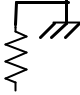
\includegraphics[width=0.37in,height=0.44in]{./media/image13.png}
\end{figure}


%%%%%%%%%%%%%%%%%%%% Figure/Image No: 10 Ends here %%%%%%%%%%%%%%%%%%%%

\par


\vspace{\baselineskip}

\vspace{\baselineskip}


%%%%%%%%%%%%%%%%%%%% Table No: 19 starts here %%%%%%%%%%%%%%%%%%%%


\begin{table}[H]
 			\centering
\begin{tabular}{p{-0.08in}p{-0.13in}p{-0.13in}p{-0.14in}p{-0.17in}p{-0.09in}p{0.09in}p{0.3in}p{-0.08in}p{-0.13in}p{-0.13in}p{-0.14in}p{0.2in}p{-0.05in}p{-0.1in}p{-0.17in}p{-0.05in}p{-0.16in}p{0.04in}}
%row no:1
\multicolumn{5}{p{-0.08in}}{\textit{\textsuperscript{V}}{\fontsize{5pt}{6.0pt}\selectfont \textit{CC}}} & 
\multicolumn{1}{p{-0.09in}}{} & 
\multicolumn{1}{p{0.09in}}{} & 
\multicolumn{1}{p{0.3in}}{} & 
\multicolumn{6}{p{-0.08in}}{{\fontsize{6pt}{7.2pt}\selectfont \textit{R\textsubscript{L}\textsuperscript{'}}}} & 
\multicolumn{1}{p{-0.1in}}{} & 
\multicolumn{1}{p{-0.17in}}{} & 
\multicolumn{1}{p{-0.05in}}{} & 
\multicolumn{1}{p{-0.16in}}{} & 
\multicolumn{1}{p{0.04in}}{} \\
\hhline{~~~~~~~~~~~~~~~~~~~}
%row no:2
\multicolumn{1}{p{-0.08in}}{} & 
\multicolumn{1}{p{-0.13in}}{} & 
\multicolumn{1}{p{-0.13in}}{} & 
\multicolumn{2}{p{0.7in}}{\multirow{1}{*}{\begin{tabular}{p{0.7in}}{\fontsize{5pt}{6.0pt}\selectfont \textit{v}}\\\end{tabular}}} & 
\multicolumn{1}{p{-0.09in}}{} & 
\multicolumn{1}{p{0.09in}}{\multirow{1}{*}{\begin{tabular}{p{0.09in}}{\fontsize{6pt}{7.2pt}\selectfont \textit{=V}}\\\end{tabular}}} & 
\multicolumn{1}{p{0.3in}}{\multirow{1}{*}{\begin{tabular}{p{0.3in}}{\fontsize{6pt}{7.2pt}\selectfont \textit{=V}}\\\end{tabular}}} & 
\multicolumn{1}{p{-0.08in}}{} & 
\multicolumn{1}{p{-0.13in}}{} & 
\multicolumn{1}{p{-0.13in}}{} & 
\multicolumn{1}{p{-0.14in}}{} & 
\multicolumn{2}{p{0.2in}}{\multirow{1}{*}{\begin{tabular}{p{0.2in}}\textit{\textsubscript{\_}}{\fontsize{5pt}{6.0pt}\selectfont \textit{\  \textsuperscript{v} CE}}\\\end{tabular}}} & 
\multicolumn{1}{p{-0.1in}}{} & 
\multicolumn{3}{p{-0.12in}}{\multirow{1}{*}{\begin{tabular}{p{-0.12in}}\textit{\textsuperscript{V}}{\fontsize{5pt}{6.0pt}\selectfont \textit{CEQ}}\\\end{tabular}}} & 
\multicolumn{1}{p{0.04in}}{\multirow{1}{*}{\begin{tabular}{p{0.04in}}{\fontsize{6pt}{7.2pt}\selectfont \textit{+ \textsuperscript{I} }{\fontsize{4pt}{4.8pt}\selectfont \textit{CQ}}}\\\end{tabular}}} \\ 

\hhline{~~~~~~~~~~~~~~~~~~~}
%row no:3
\multicolumn{1}{p{-0.08in}}{} & 
\multicolumn{1}{p{-0.13in}}{} & 
\multicolumn{1}{p{-0.13in}}{} & 
\multicolumn{2}{p{0.7in}}{} & 
\multicolumn{1}{p{-0.09in}}{} & 
\multicolumn{1}{p{0.09in}}{} & 
\multicolumn{1}{p{0.3in}}{} & 
\multicolumn{1}{p{-0.08in}}{} & 
\multicolumn{1}{p{-0.13in}}{} & 
\multicolumn{1}{p{-0.13in}}{} & 
\multicolumn{1}{p{-0.14in}}{} & 
\multicolumn{2}{p{0.2in}}{} & 
\multicolumn{1}{p{-0.1in}}{} & 
\multicolumn{3}{p{-0.12in}}{} & 
\multicolumn{1}{p{0.04in}}{} \\
\hhline{~~~~~~~~~~~~~~~~~~~}
%row no:4
\multicolumn{1}{p{-0.08in}}{} & 
\multicolumn{1}{p{-0.13in}}{} & 
\multicolumn{1}{p{-0.13in}}{} & 
\multicolumn{1}{p{-0.14in}}{} & 
\multicolumn{1}{p{-0.17in}}{} & 
\multicolumn{1}{p{-0.09in}}{{\fontsize{4pt}{4.8pt}\selectfont \textit{CE}}} & 
\multicolumn{1}{p{0.09in}}{{\fontsize{4pt}{4.8pt}\selectfont \textit{CEQ}}} & 
\multicolumn{1}{p{0.3in}}{{\fontsize{4pt}{4.8pt}\selectfont \textit{CC}}} & 
\multicolumn{1}{p{-0.08in}}{} & 
\multicolumn{1}{p{-0.13in}}{} & 
\multicolumn{1}{p{-0.13in}}{} & 
\multicolumn{1}{p{-0.14in}}{} & 
\multicolumn{1}{p{0.2in}}{{\fontsize{4pt}{4.8pt}\selectfont \textit{i \textsubscript{C}\ \  =}}} & 
\multicolumn{1}{p{-0.05in}}{\multirow{1}{*}{\begin{tabular}{p{-0.05in}}{\fontsize{5pt}{6.0pt}\selectfont \textit{R\textsubscript{L}\textsuperscript{'}}}\\\end{tabular}}} & 
\multicolumn{1}{p{-0.1in}}{{\fontsize{5pt}{6.0pt}\selectfont \textit{+}}} & 
\multicolumn{1}{p{-0.17in}}{} & 
\multicolumn{1}{p{-0.05in}}{\multirow{1}{*}{\begin{tabular}{p{-0.05in}}{\fontsize{5pt}{6.0pt}\selectfont \textit{R\textsubscript{L}\textsuperscript{'}}}\\\end{tabular}}} & 
\multicolumn{1}{p{-0.16in}}{\multirow{1}{*}{\begin{tabular}{p{-0.16in}}\end{tabular}}} & 
\multicolumn{1}{p{0.04in}}{} \\
\hhline{~~~~~~~~~~~~~~~~~~~}
%row no:5
\multicolumn{1}{p{-0.08in}}{} & 
\multicolumn{1}{p{-0.13in}}{} & 
\multicolumn{1}{p{-0.13in}}{} & 
\multicolumn{1}{p{-0.14in}}{} & 
\multicolumn{1}{p{-0.17in}}{} & 
\multicolumn{1}{p{-0.09in}}{} & 
\multicolumn{1}{p{0.09in}}{} & 
\multicolumn{1}{p{0.3in}}{} & 
\multicolumn{1}{p{-0.08in}}{} & 
\multicolumn{1}{p{-0.13in}}{} & 
\multicolumn{1}{p{-0.13in}}{} & 
\multicolumn{1}{p{-0.14in}}{} & 
\multicolumn{1}{p{0.2in}}{} & 
\multicolumn{1}{p{-0.05in}}{} & 
\multicolumn{1}{p{-0.1in}}{} & 
\multicolumn{1}{p{-0.17in}}{} & 
\multicolumn{1}{p{-0.05in}}{} & 
\multicolumn{1}{p{-0.16in}}{} & 
\multicolumn{1}{p{0.04in}}{} \\
\hhline{~~~~~~~~~~~~~~~~~~~}
%row no:6
\multicolumn{1}{p{-0.08in}}{} & 
\multicolumn{1}{p{-0.13in}}{} & 
\multicolumn{1}{p{-0.13in}}{} & 
\multicolumn{1}{p{-0.14in}}{} & 
\multicolumn{1}{p{-0.17in}}{} & 
\multicolumn{1}{p{-0.09in}}{} & 
\multicolumn{1}{p{0.09in}}{} & 
\multicolumn{1}{p{0.3in}}{} & 
\multicolumn{1}{p{-0.08in}}{} & 
\multicolumn{1}{p{-0.13in}}{} & 
\multicolumn{1}{p{-0.13in}}{} & 
\multicolumn{1}{p{-0.14in}}{} & 
\multicolumn{1}{p{0.2in}}{} & 
\multicolumn{1}{p{-0.05in}}{} & 
\multicolumn{1}{p{-0.1in}}{} & 
\multicolumn{1}{p{-0.17in}}{} & 
\multicolumn{1}{p{-0.05in}}{} & 
\multicolumn{1}{p{-0.16in}}{} & 
\multicolumn{1}{p{0.04in}}{} \\
\hhline{~~~~~~~~~~~~~~~~~~~}
%row no:7
\multicolumn{1}{p{-0.08in}}{} & 
\multicolumn{4}{p{-0.12in}}{{\fontsize{6pt}{7.2pt}\selectfont (a)}} & 
\multicolumn{1}{p{-0.09in}}{} & 
\multicolumn{1}{p{0.09in}}{} & 
\multicolumn{1}{p{0.3in}}{} & 
\multicolumn{1}{p{-0.08in}}{} & 
\multicolumn{1}{p{-0.13in}}{} & 
\multicolumn{1}{p{-0.13in}}{} & 
\multicolumn{1}{p{-0.14in}}{} & 
\multicolumn{2}{p{0.2in}}{{\fontsize{6pt}{7.2pt}\selectfont (b)}} & 
\multicolumn{1}{p{-0.1in}}{} & 
\multicolumn{1}{p{-0.17in}}{} & 
\multicolumn{1}{p{-0.05in}}{} & 
\multicolumn{1}{p{-0.16in}}{} & 
\multicolumn{1}{p{0.04in}}{} \\
\hhline{~~~~~~~~~~~~~~~~~~~}

\end{tabular}
 \end{table}


%%%%%%%%%%%%%%%%%%%% Table No: 19 ends here %%%%%%%%%%%%%%%%%%%%



%%%%%%%%%%%%%%%%%%%% Figure/Image No: 11 starts here %%%%%%%%%%%%%%%%%%%%


\begin{figure}[H]	\begin{subfigure}		
\includegraphics[width=0.12\textwidth]{./media/image14.png}
	\end{subfigure}
~	\begin{subfigure}		
\includegraphics[width=0.12\textwidth]{./media/image15.png}
	\end{subfigure}
~	\begin{subfigure}		
\includegraphics[width=0.12\textwidth]{./media/image14.png}
	\end{subfigure}
~	\begin{subfigure}		
\includegraphics[width=0.12\textwidth]{./media/image15.png}
	\end{subfigure}
~	\begin{subfigure}		
\includegraphics[width=0.12\textwidth]{./media/image16.png}
	\end{subfigure}
~	\begin{subfigure}		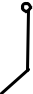
\includegraphics[width=0.12\textwidth]{./media/image17.png}
	\end{subfigure}
~
\end{figure}


%%%%%%%%%%%%%%%%%%%% Figure/Image No: 11 Ends here %%%%%%%%%%%%%%%%%%%%

\par


\vspace{\baselineskip}
\begin{adjustwidth}{0.0in}{0.01in}
\begin{Center}
Figure 7: Equivalentes de CC y CA
\end{Center}\par

\end{adjustwidth}


\vspace{\baselineskip}

\vspace{\baselineskip}

\vspace{\baselineskip}

\vspace{\baselineskip}

\printbibliography
\end{document}